\documentclass[12pt,a4paper]{article}
\usepackage[utf8]{inputenc}
\usepackage{graphicx}   % Para insertar gráficos
\usepackage{geometry}   % Para márgenes
\geometry{top=2.5cm, bottom=2.5cm, left=2.5cm, right=2.5cm}
\usepackage{setspace}   % Para controlar espacio entre líneas
\usepackage{lipsum}     % Solo para texto de ejemplo
\renewcommand{\contentsname}{Contenidos}

% ---------------- Caratula ----------------
\begin{document}
\begin{titlepage}
    \centering
    \vspace*{2cm}
    
    {\Huge \textbf{Alix Partners: La Casa de Asterión}}\\[0.5cm]
    {\Large Predicción de demanda y optimización de precios}\\[1.5cm]
    
    {\Large 2025}\\[2cm]

\end{titlepage}

% ---------------- Contenido ----------------
\tableofcontents
\newpage

\section{Introducción}

En esta competencia, nos fue dado el siguiente desafío: un negocio de ventas minoristas, llamado "La Casa de Asterión", ha sufrido una reducción de ganancias 
en el último tiempo, y necesita mejorar su estrategia de precios para solucionar este problema. La empresa ha proporcionado los siguientes datos: las transacciones 
de ventas de los últimos 3 años, especificando las tiendas, los productos vendidos y sus precios. Además, también contamos con datos sobre las tiendas, como su ubicación, 
y sobre los productos, como su categoría y marca. 

\vspace{0.2cm}

Entonces, valiéndonos de toda esta información, nuestro objetivo es contruir un modelo capaz de predecir la demanda diaria de los prodcutos de la próxima semana a 
partir del precio y otras variables, y con el mismo, optimizar los precios para maximizar las ganancias.

\vspace{0.2cm}

Dado que desconocemos si el cliente tiene conocimientos técnicos acerca de programación y desarrollo de modelos de AI, 
hemos decidido dividir este informe en dos secciones: por un lado, un análisis económico, el cual no necesita conocimientos técnicos para ser entendido, 
donde realizamos un análisis de datos básico y exponemos una estrategia de precios que, según las predicciones hechas, debería aumentar las ganancias; 
y por otro lado, realizamos un análisis técnico, en donde detallamos el preprocesamiento de datos, la construcción y entrenamiento de los modelos predictivos, 
la metodología de optimización de precios y una interpretación del mejor modelo entrenado.

\vspace{0.2cm}

Además, todo el código fuente utilizado para el trabajo está disponible adjunto al informe.



\newpage

\section{Análisis Económico}

En primer lugar, nos preguntamos por qué se ha producido una caída de las ganancias y qué tan grave es. Para esto, se puede observar 
en el siguiente gráfico cómo fue evolucionando la ganancia total de la empresa a lo largo del tiempo, y cómo la misma ha ido disminuyendo de a poco 
en el transcurso del tiempo.
\begin{center}
    \makebox[\textwidth][c]{%
        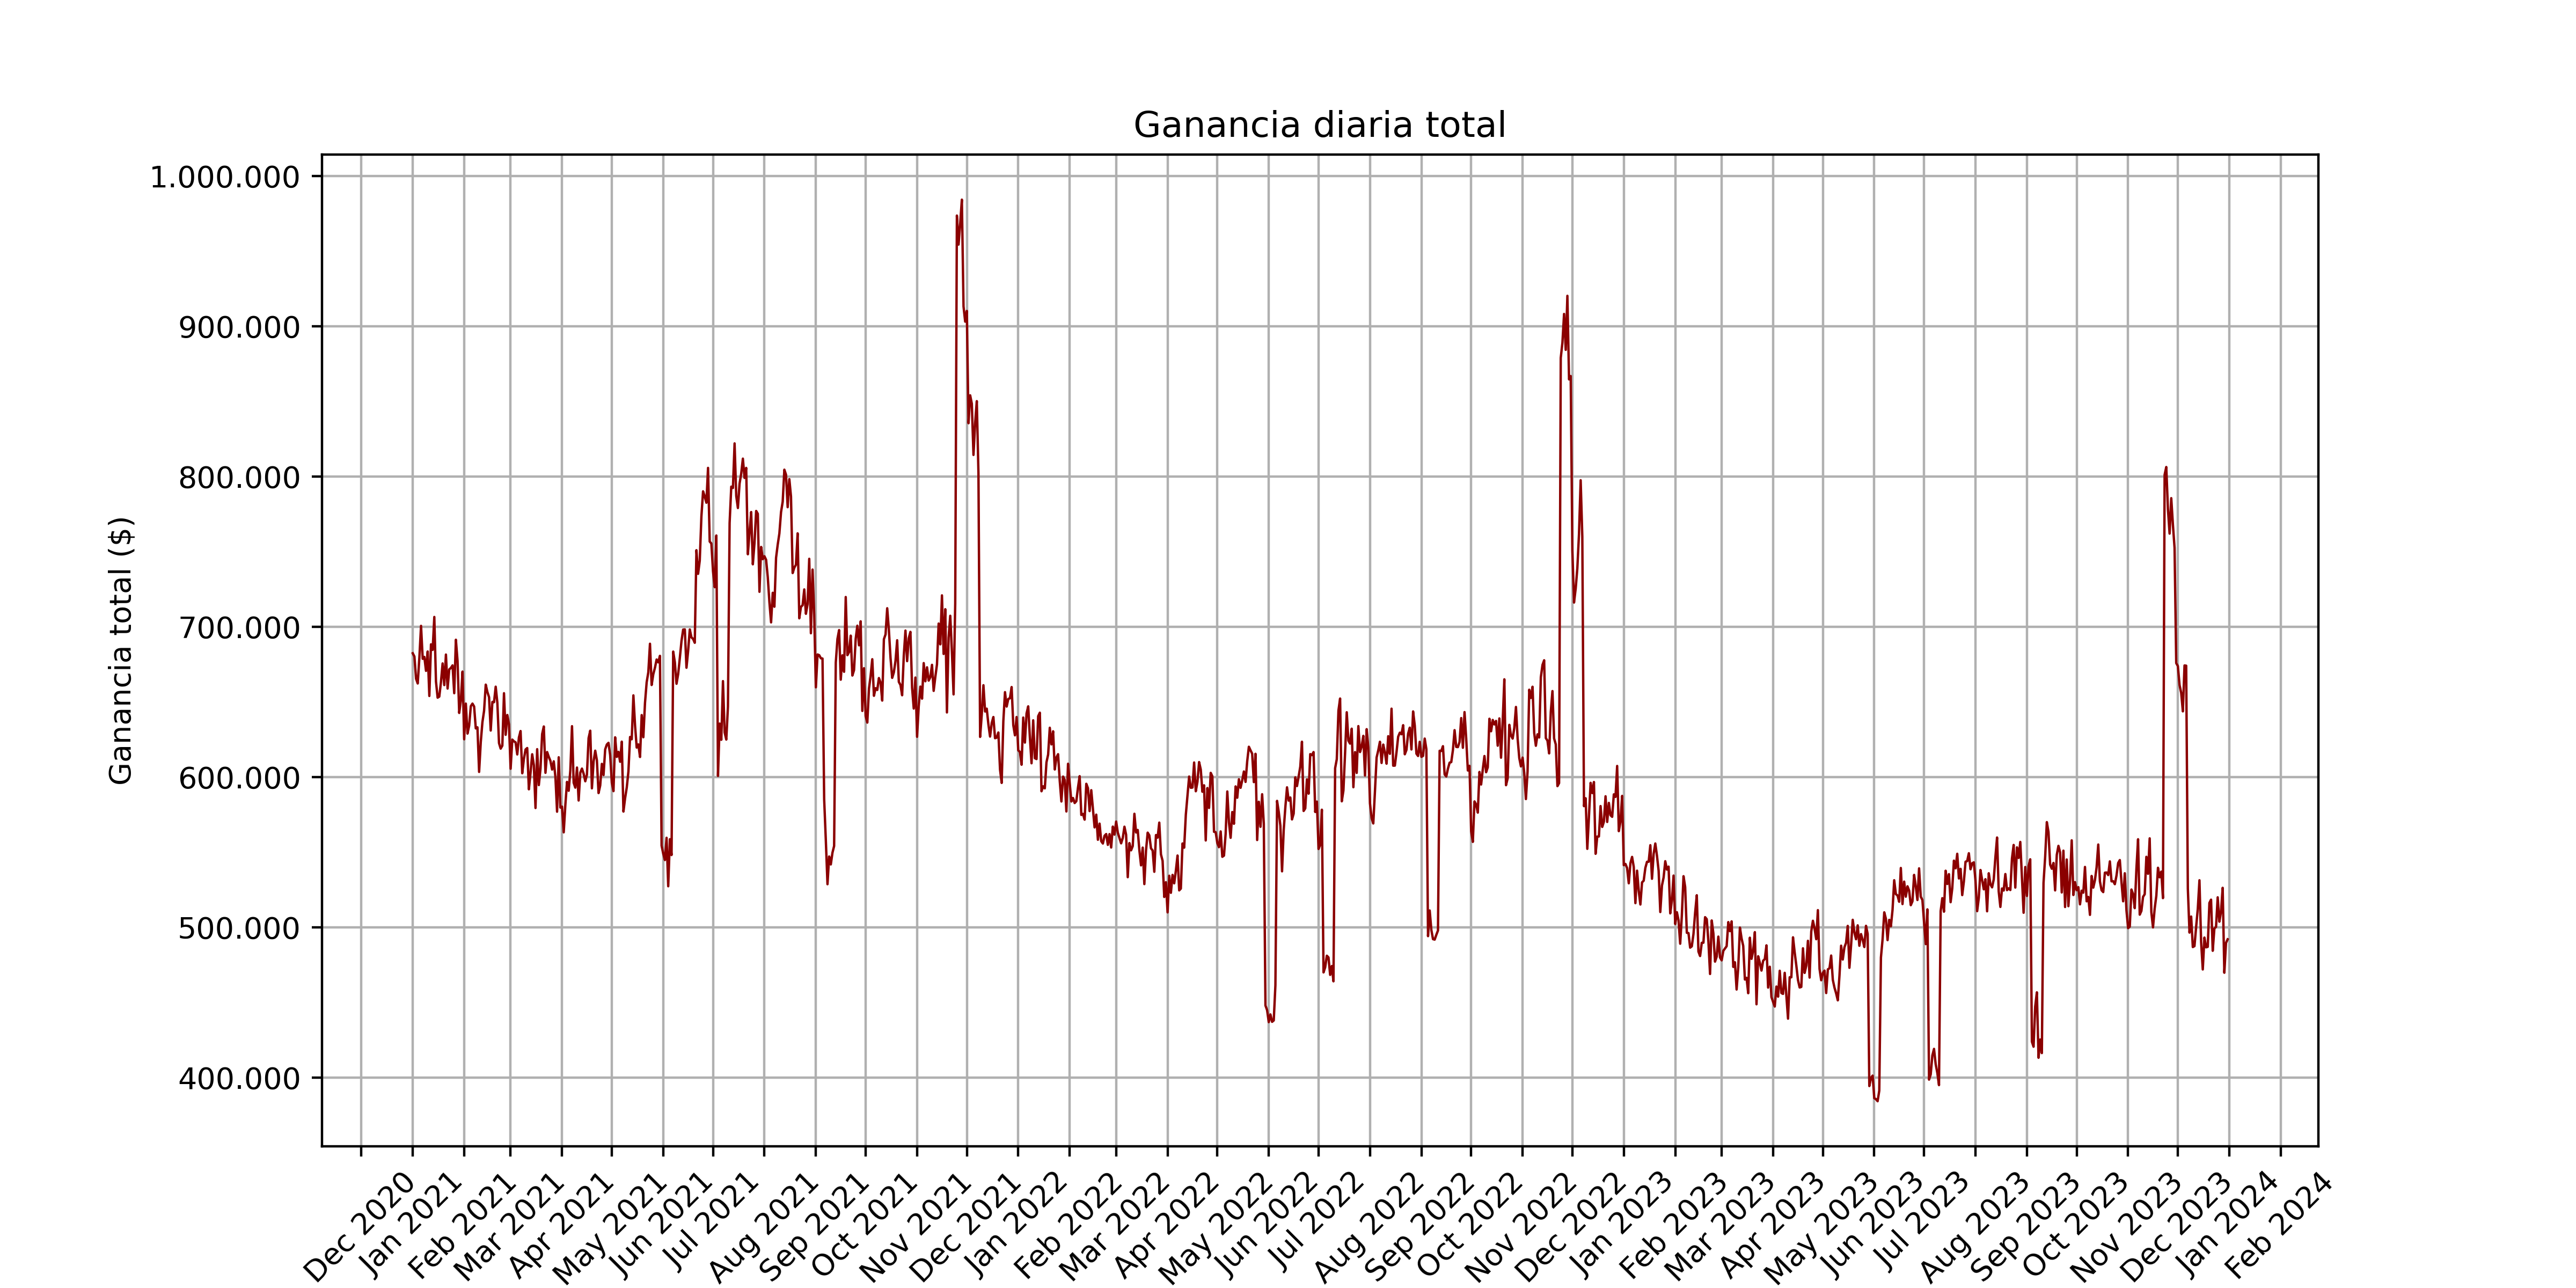
\includegraphics[width=1.1\textwidth]{graficos/ganancia_diaria_total.png}%
    }
\end{center}

En concreto, con respecto al primer año, las ganancias totales se han reducido un 11.3\% en el segundo año y un 23.7\% en el tercer año, 
lo cual puede resultar preocupante.

\vspace{0.2cm}

Este fenómeno puede deberse en gran parte a la reducción de la demanda total, que ha disminuído 10\% el primer año y un 21.2\% en el segundo año. 
Esto se puede apreciar en el siguiente gráfico, además de cómo varía la demanda según la categoría de los productos:
\begin{center}
    \makebox[\textwidth][c]{%
        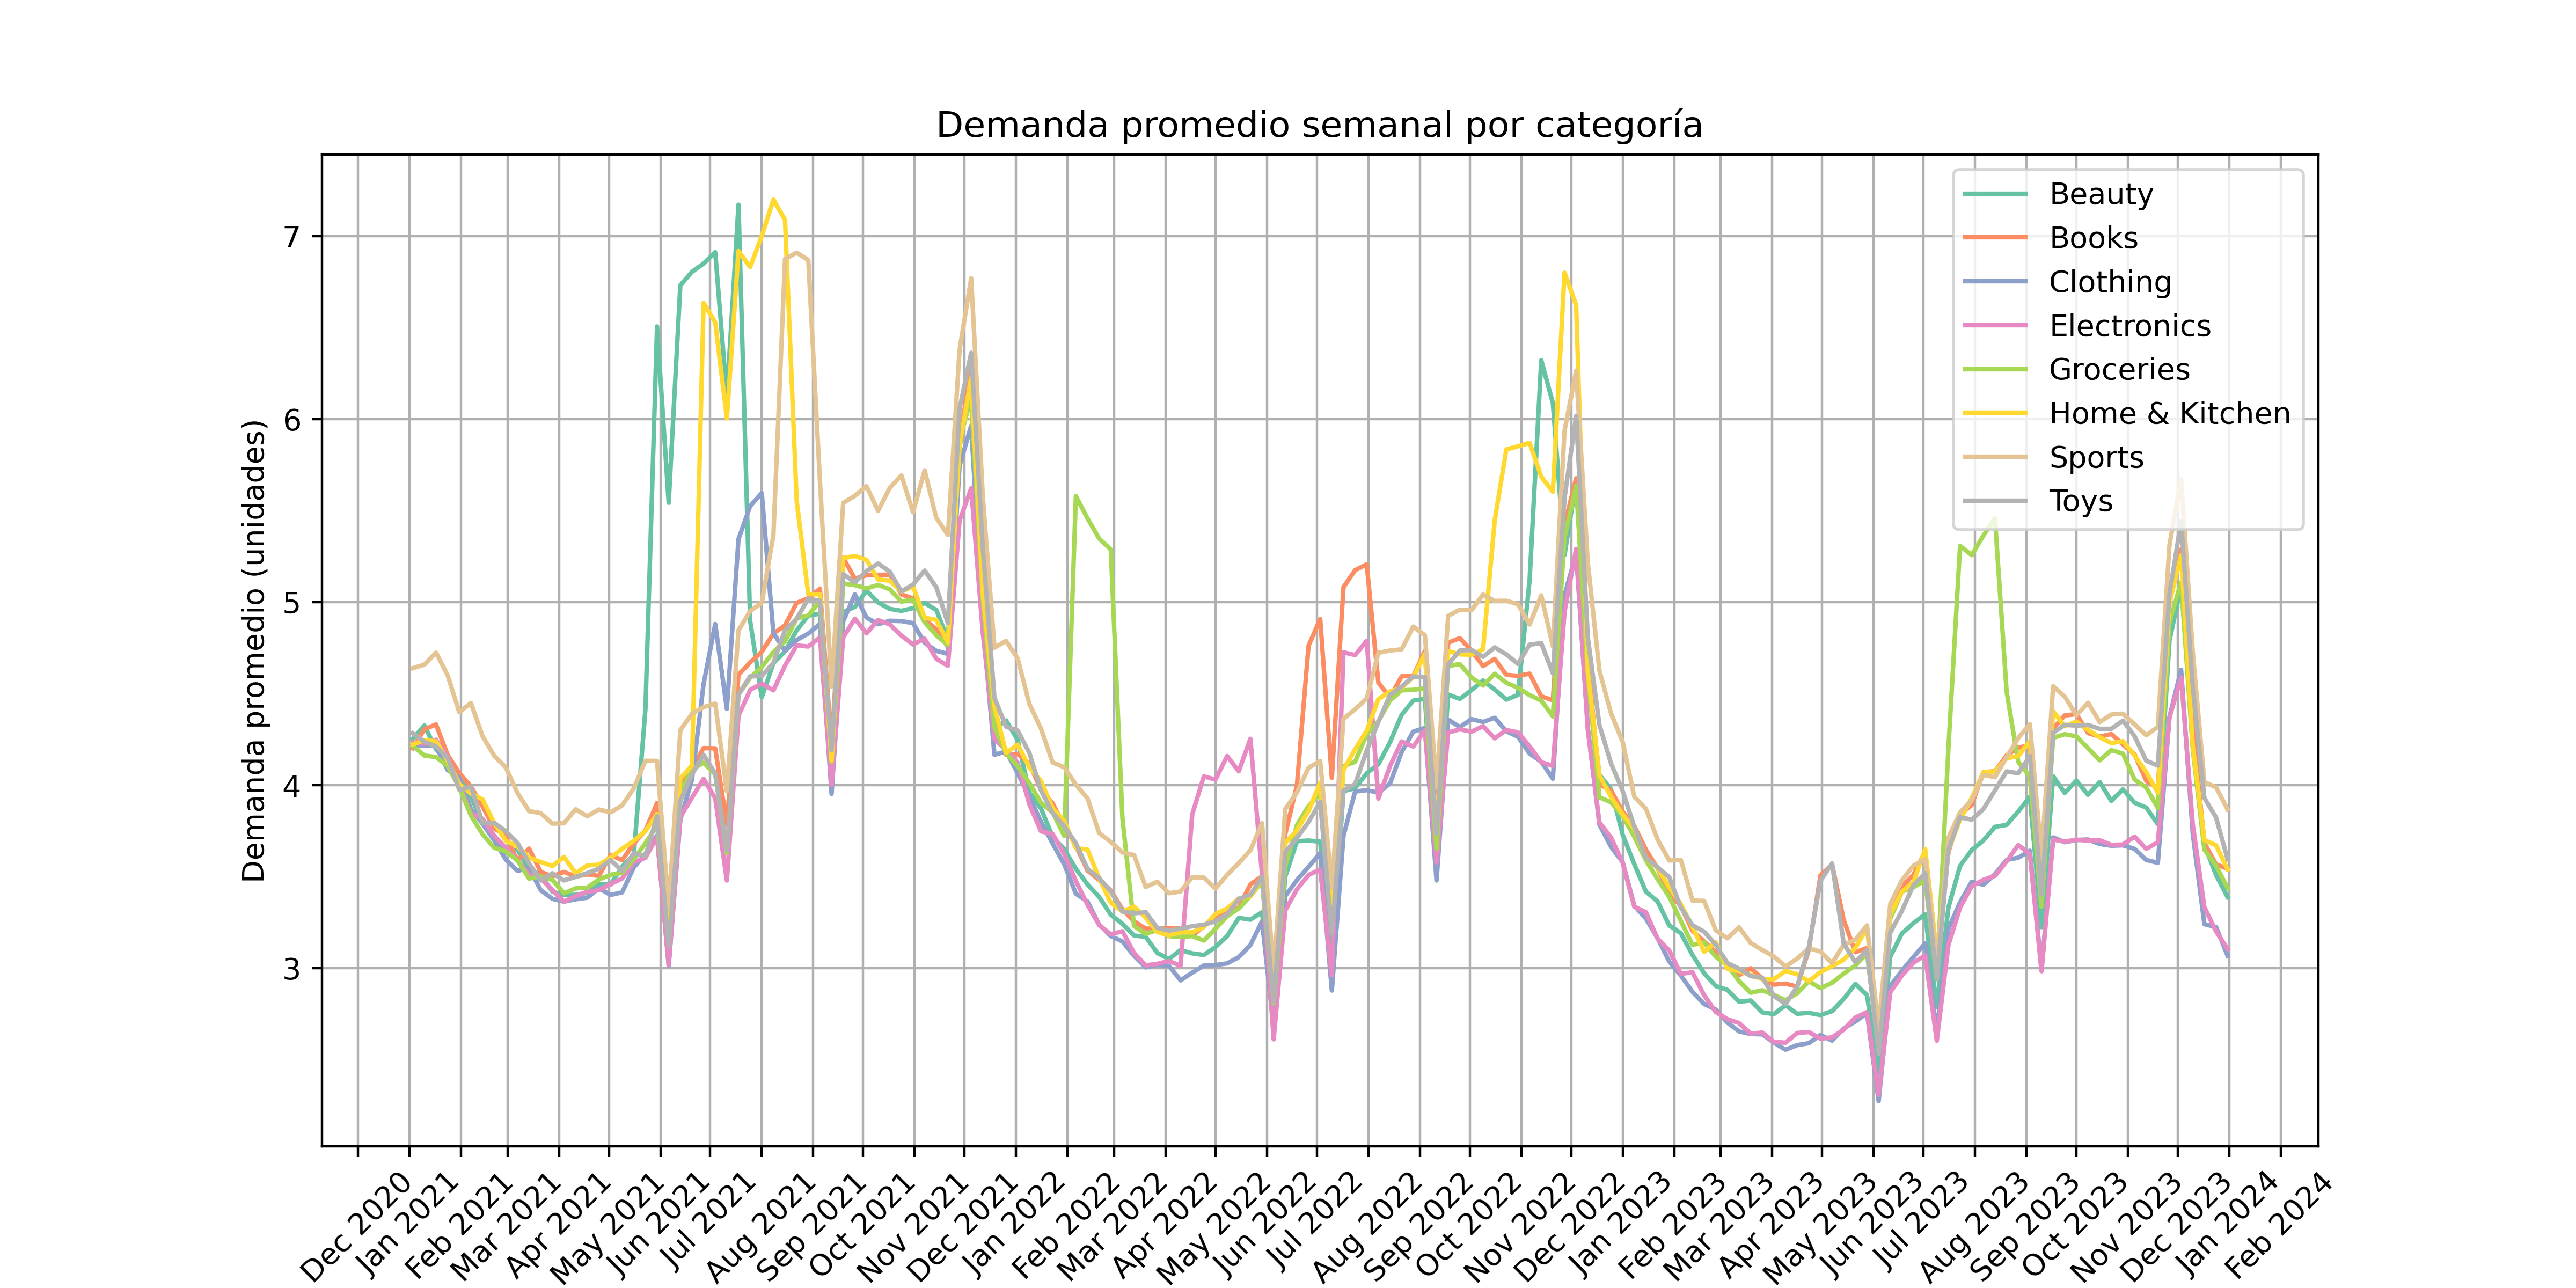
\includegraphics[width=1.2\textwidth]{graficos/demanda_promedio_semanal_por_categoria.png}%
    }
\end{center}

Al comparar este último gráfico con el de las ganancias totales, se pueden observar 3 comportamientos similares: 
\begin{itemize}
    \item A nivel global, hay una reducción gradual de las ganancias y la demanda.
    \item En cada año, en general hay un incremento a medida que transcurre el año y un descenso a principios de cada año.
    \item En Mayo, Junio y Agosto hay caídas abruptas, mientras que en Diciembre hay un incremento sustancial, seguramente debido a las festividades.
\end{itemize}

Decidimos analizar si estos descensos en la demanda se debían a cambios en los precios, sin embargo, en el siguiente gráfico se aprecia 
que en promedio los precios han seguido un mismo patrón:

\begin{center}
    \makebox[\textwidth][c]{%
        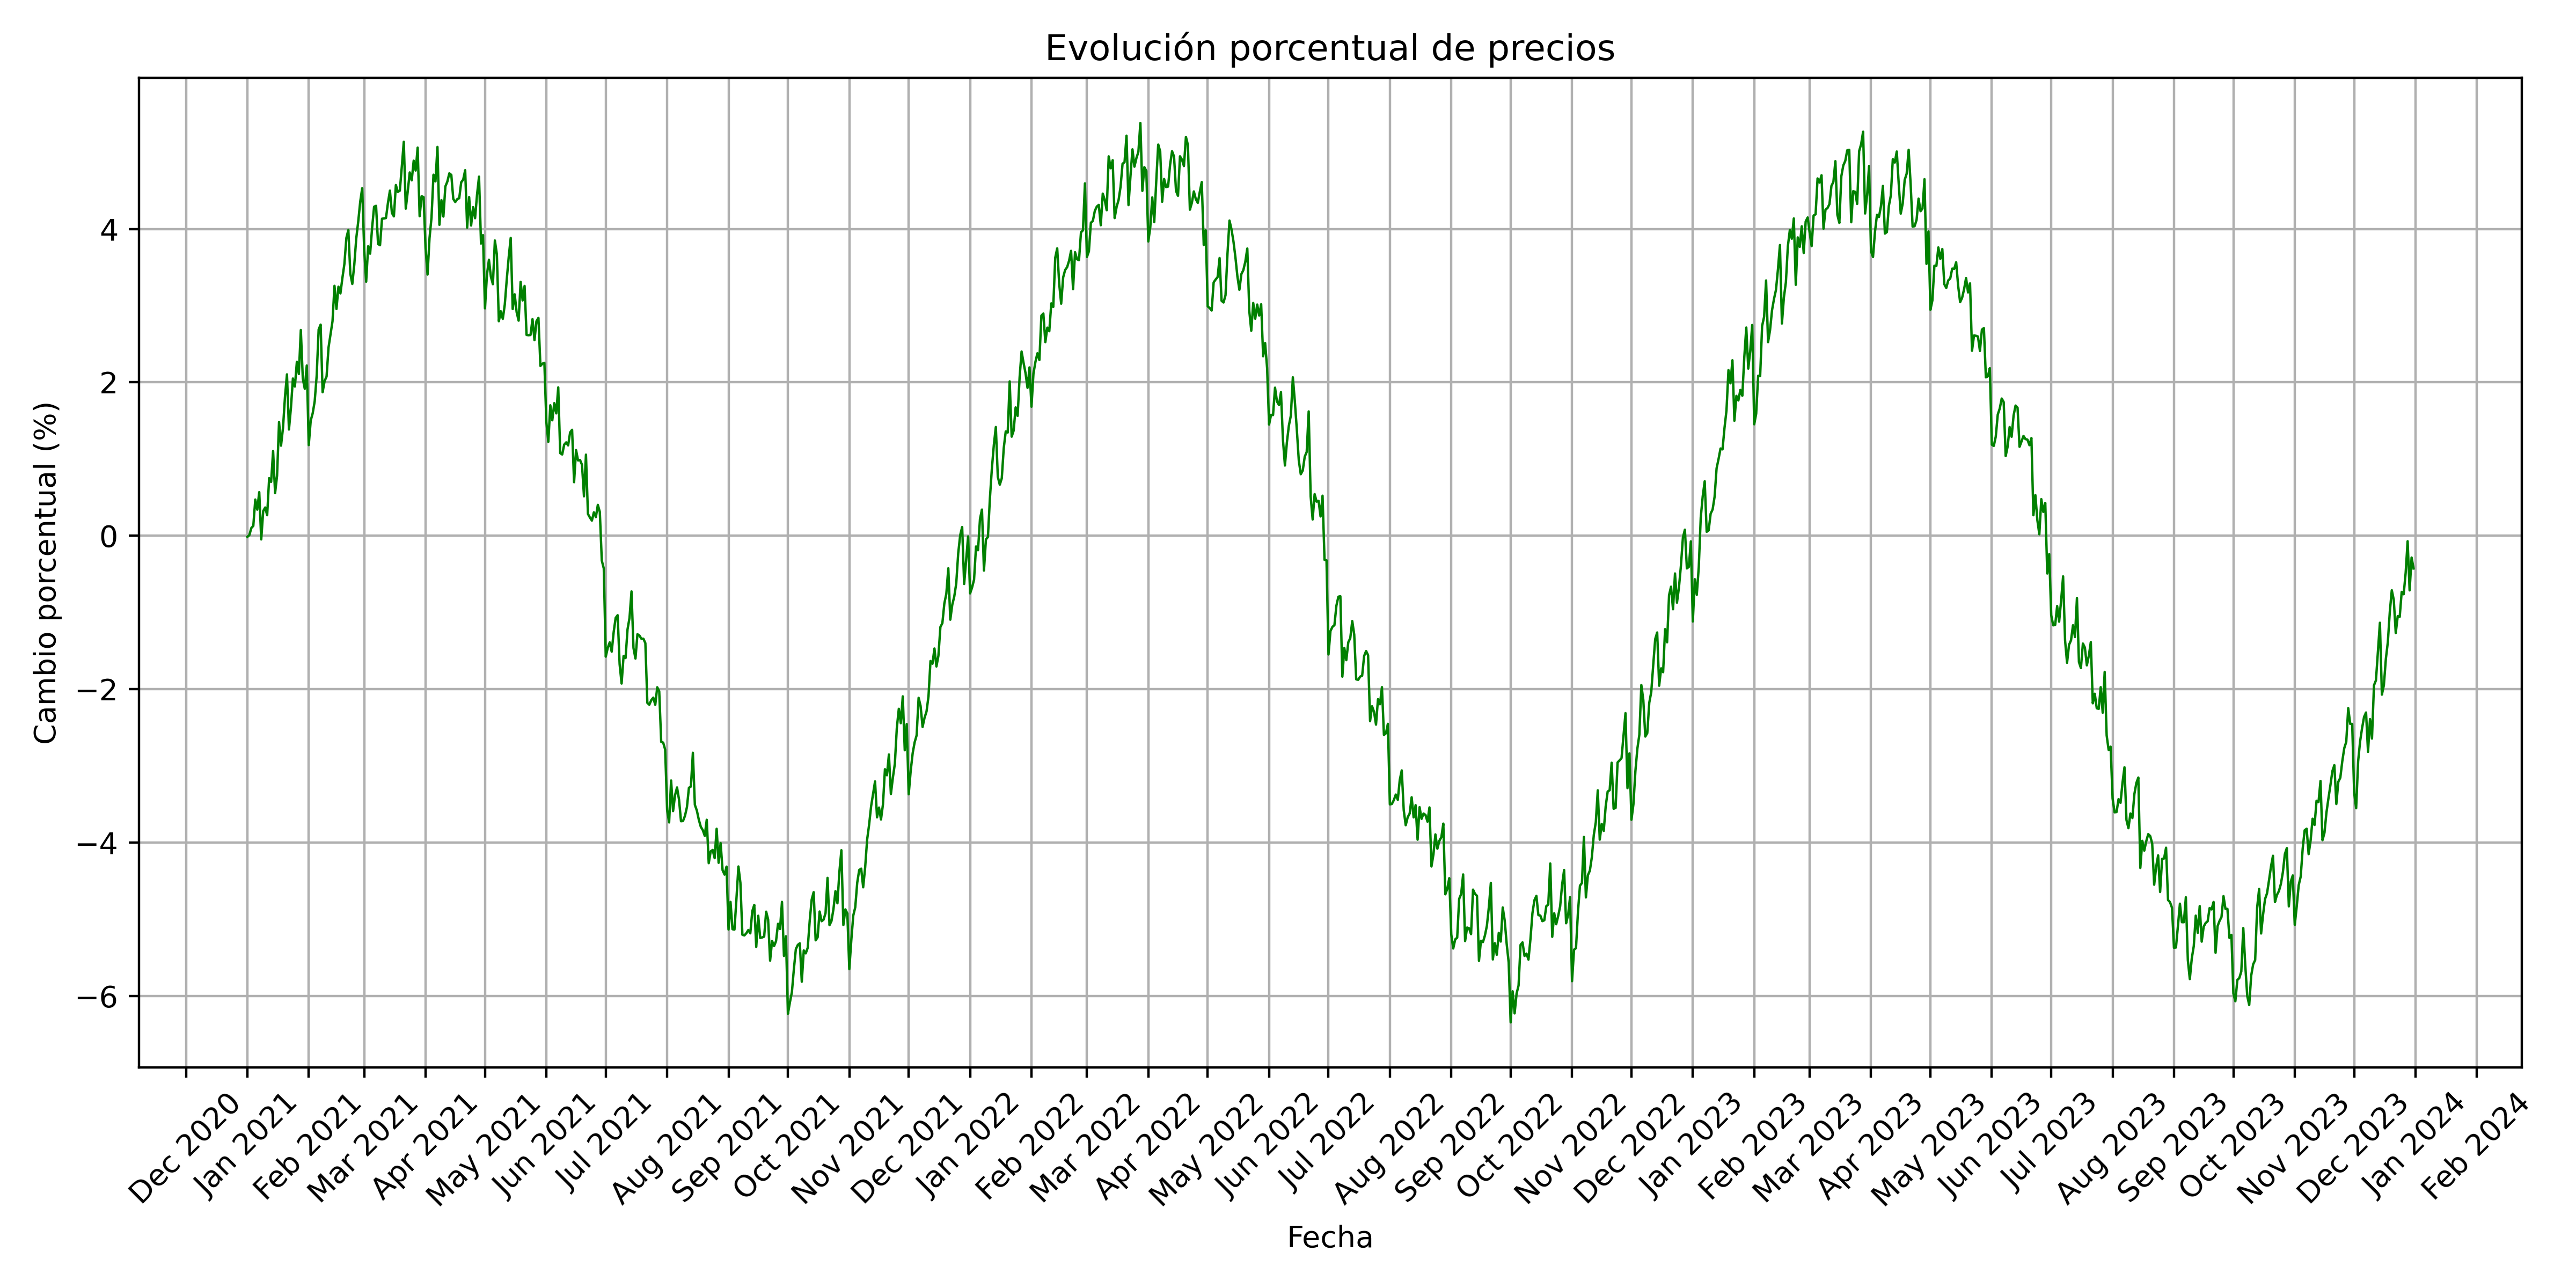
\includegraphics[width=1\textwidth]{graficos/evolucion_porcentual_precios.png}%
    }
\end{center}

Dado que los precios en general no han variado pero la demanda sí, nos lleva a pensar que es posible que un factor 
importante en la reducción sea la estrategia de precios actual, la cual no aprovecha correctamente 
la estacionalidad de la demanda. De hecho, en cada uno de los productos podemos 
observar un comportamiento similar: los precios oscilan de manera periódica a lo largo del año, pero en ciertos 
momentos, hay caídas abruptas en los precios, como se muestra a continuación.

\begin{center}
    \makebox[\textwidth][c]{%
        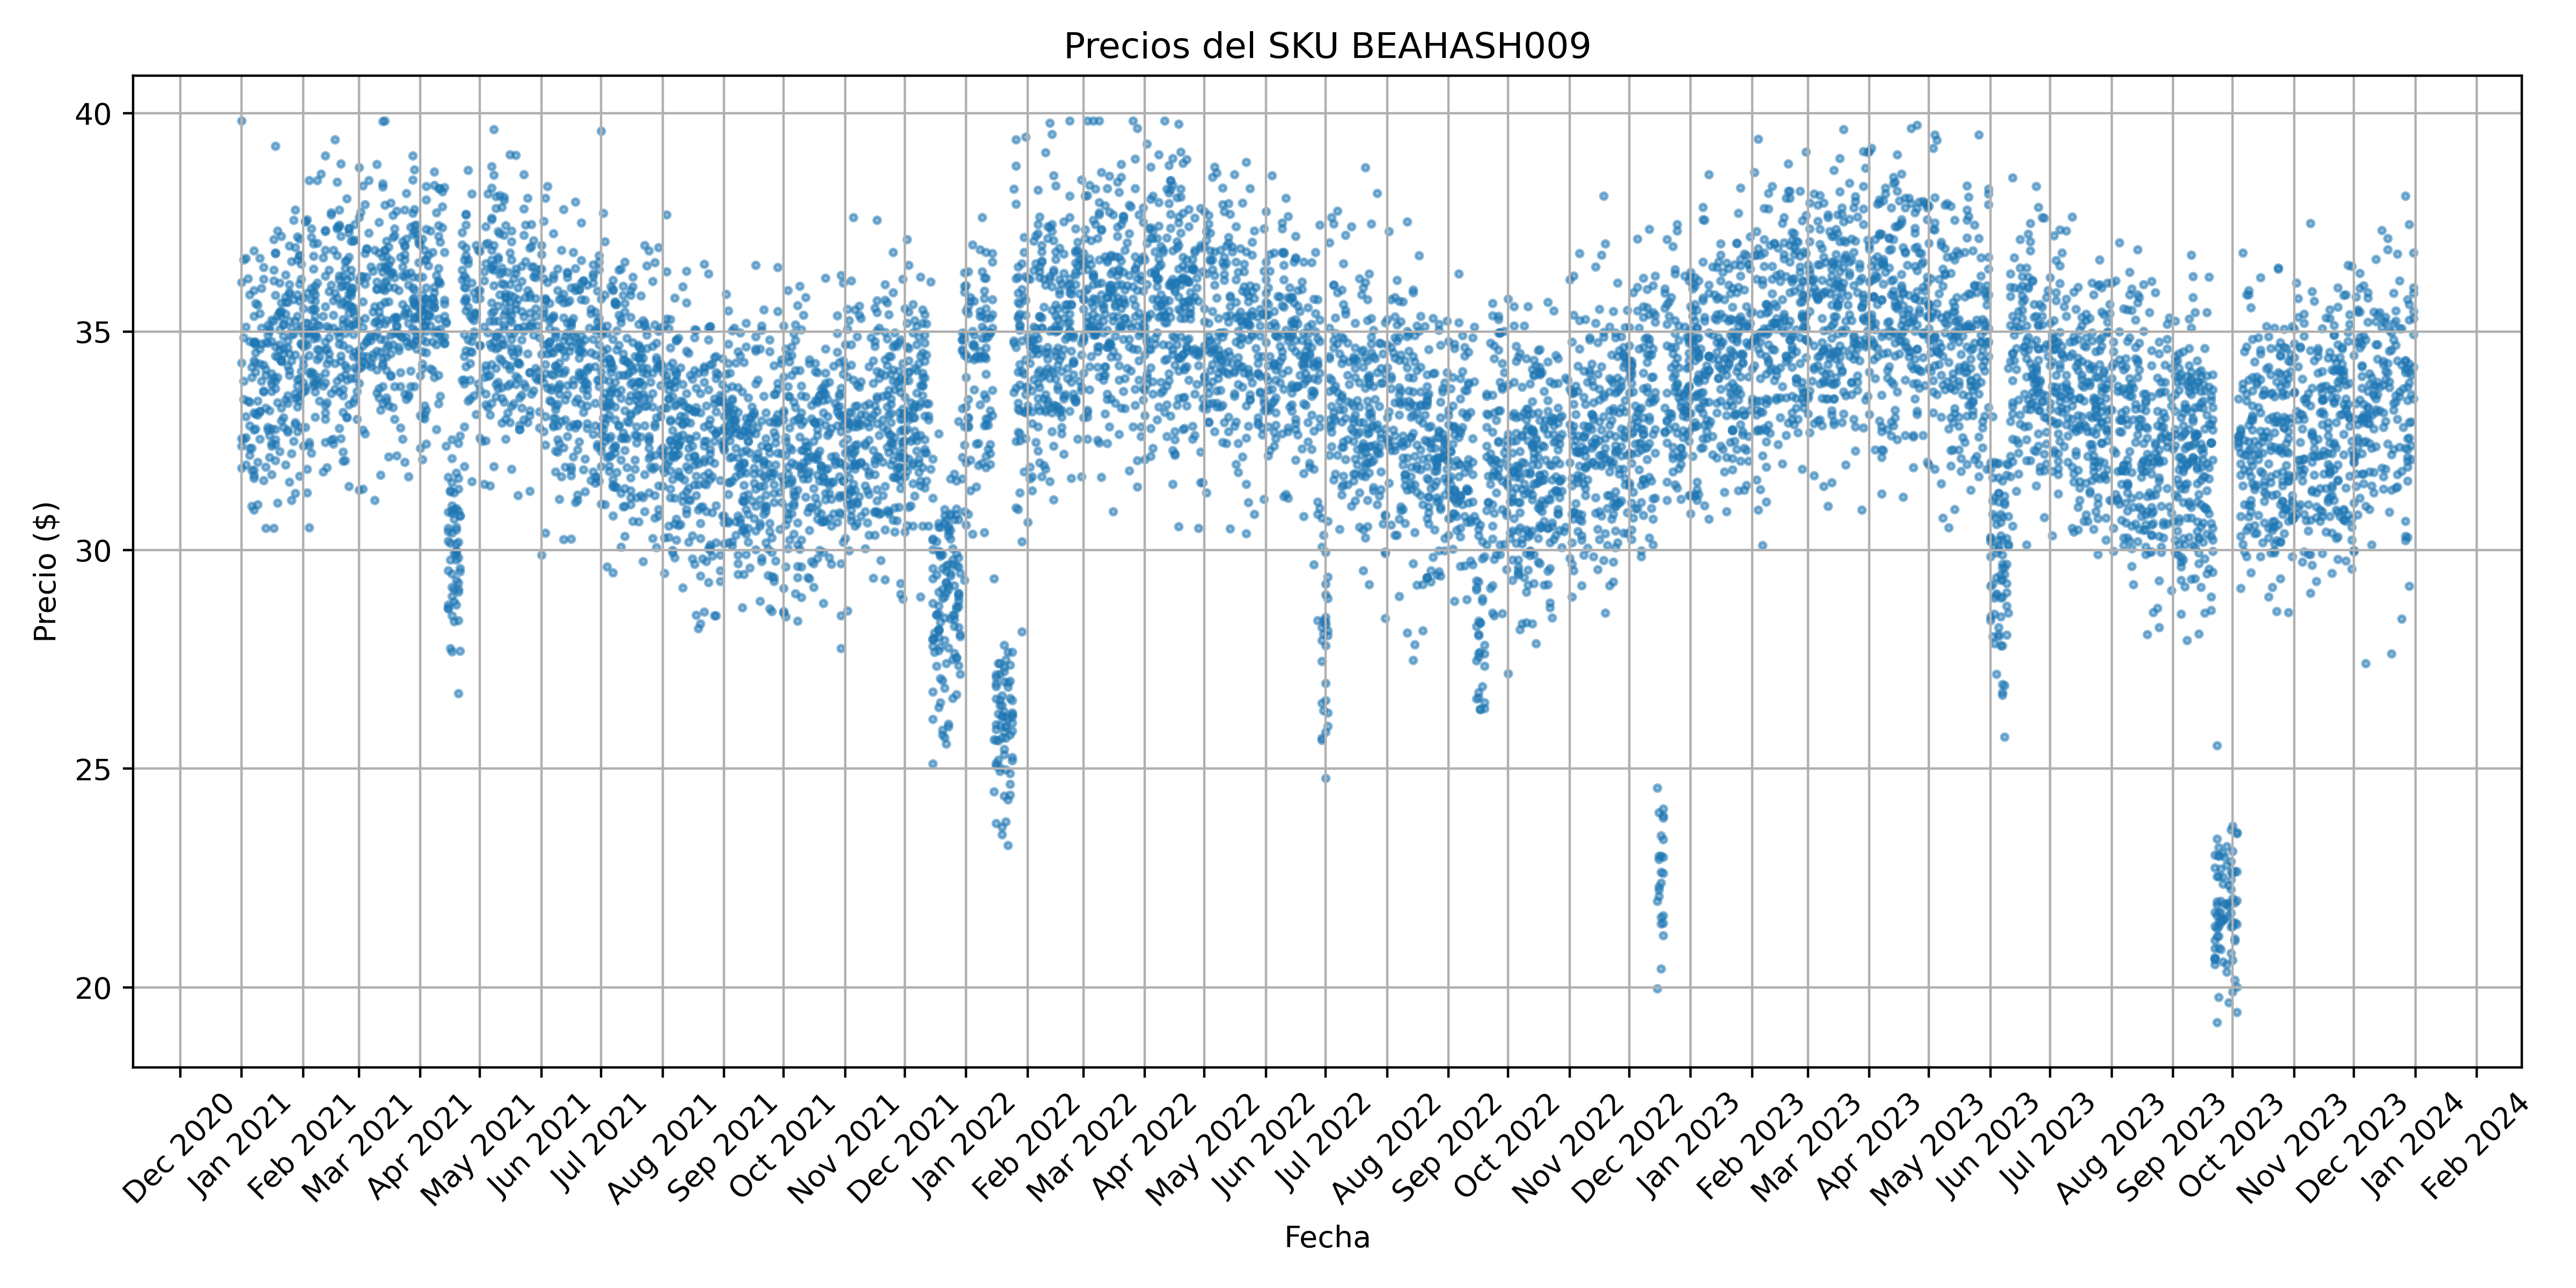
\includegraphics[width=0.8\textwidth]{graficos/precios_sku_BEAHASH009.png}%
    }
\end{center}

Por otro lado, la disminución de la demanda de diferentes productos no afecta a las ganancias de la misma 
manera, puesto que las ganancias están constituídas mayormente por productos de la categoría de electrónica:

\begin{center}
    \makebox[\textwidth][c]{%
        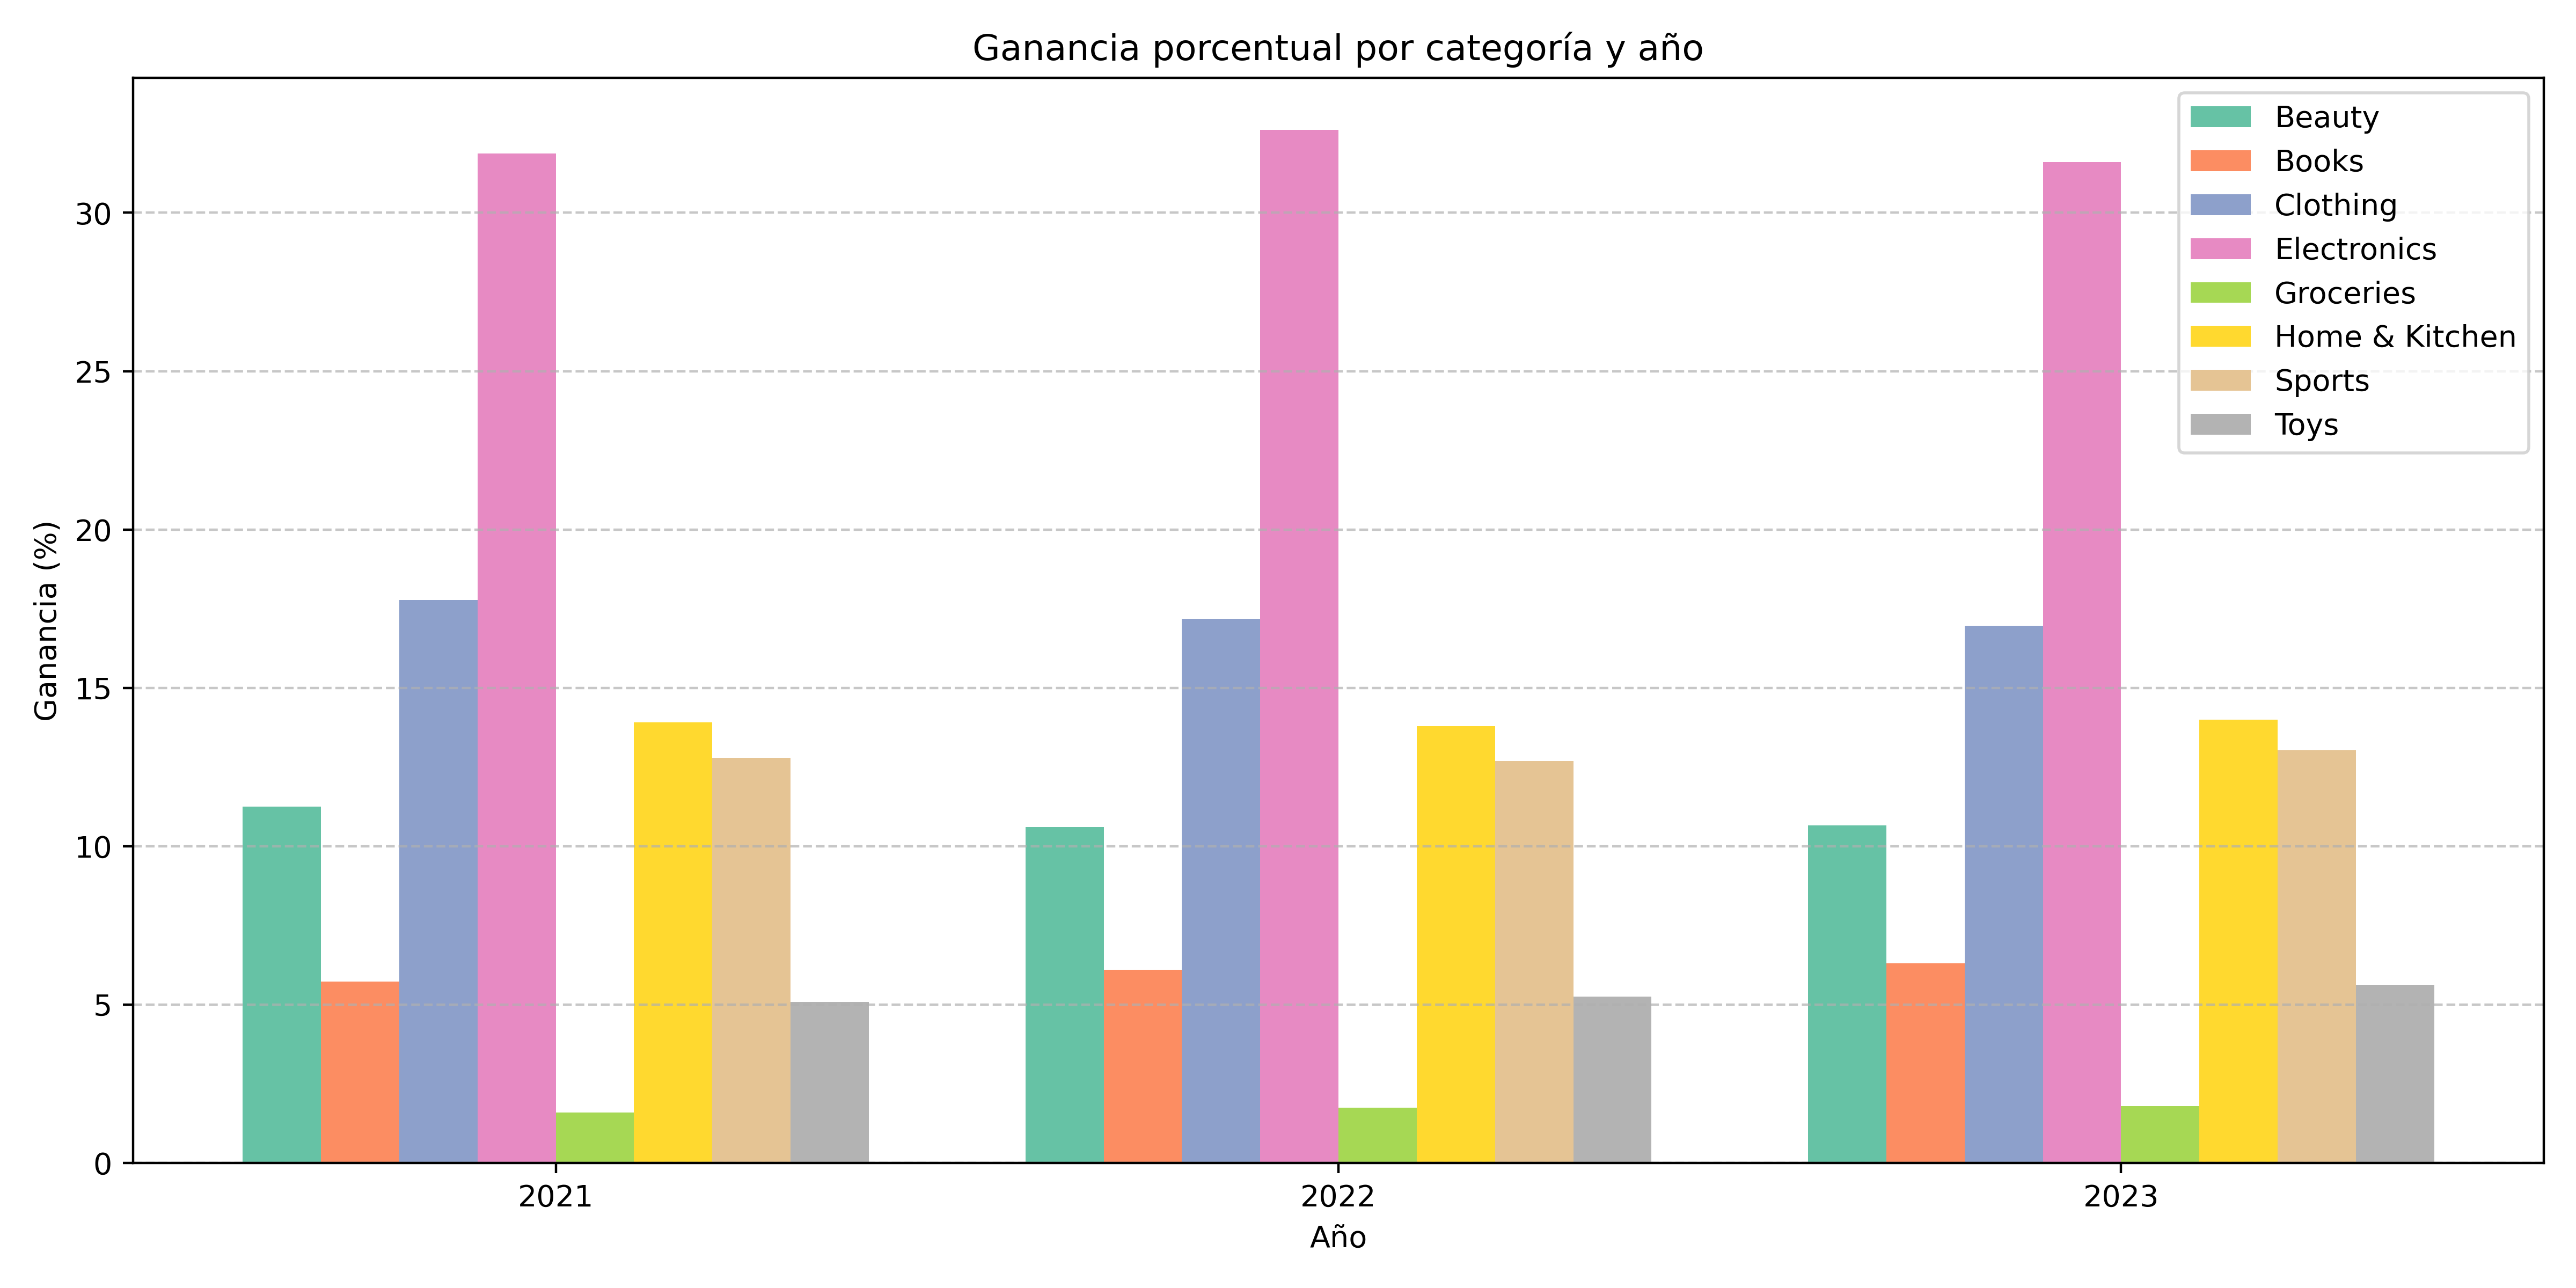
\includegraphics[width=0.8\textwidth]{graficos/ganancia_porcentual_por_categoria.png}%
    }
\end{center}

Cabe resaltar también que hay un gran desbalance de las ganancias por región y que el mismo 
se mantiene en todos los años:

\begin{center}
    \makebox[\textwidth][c]{%
        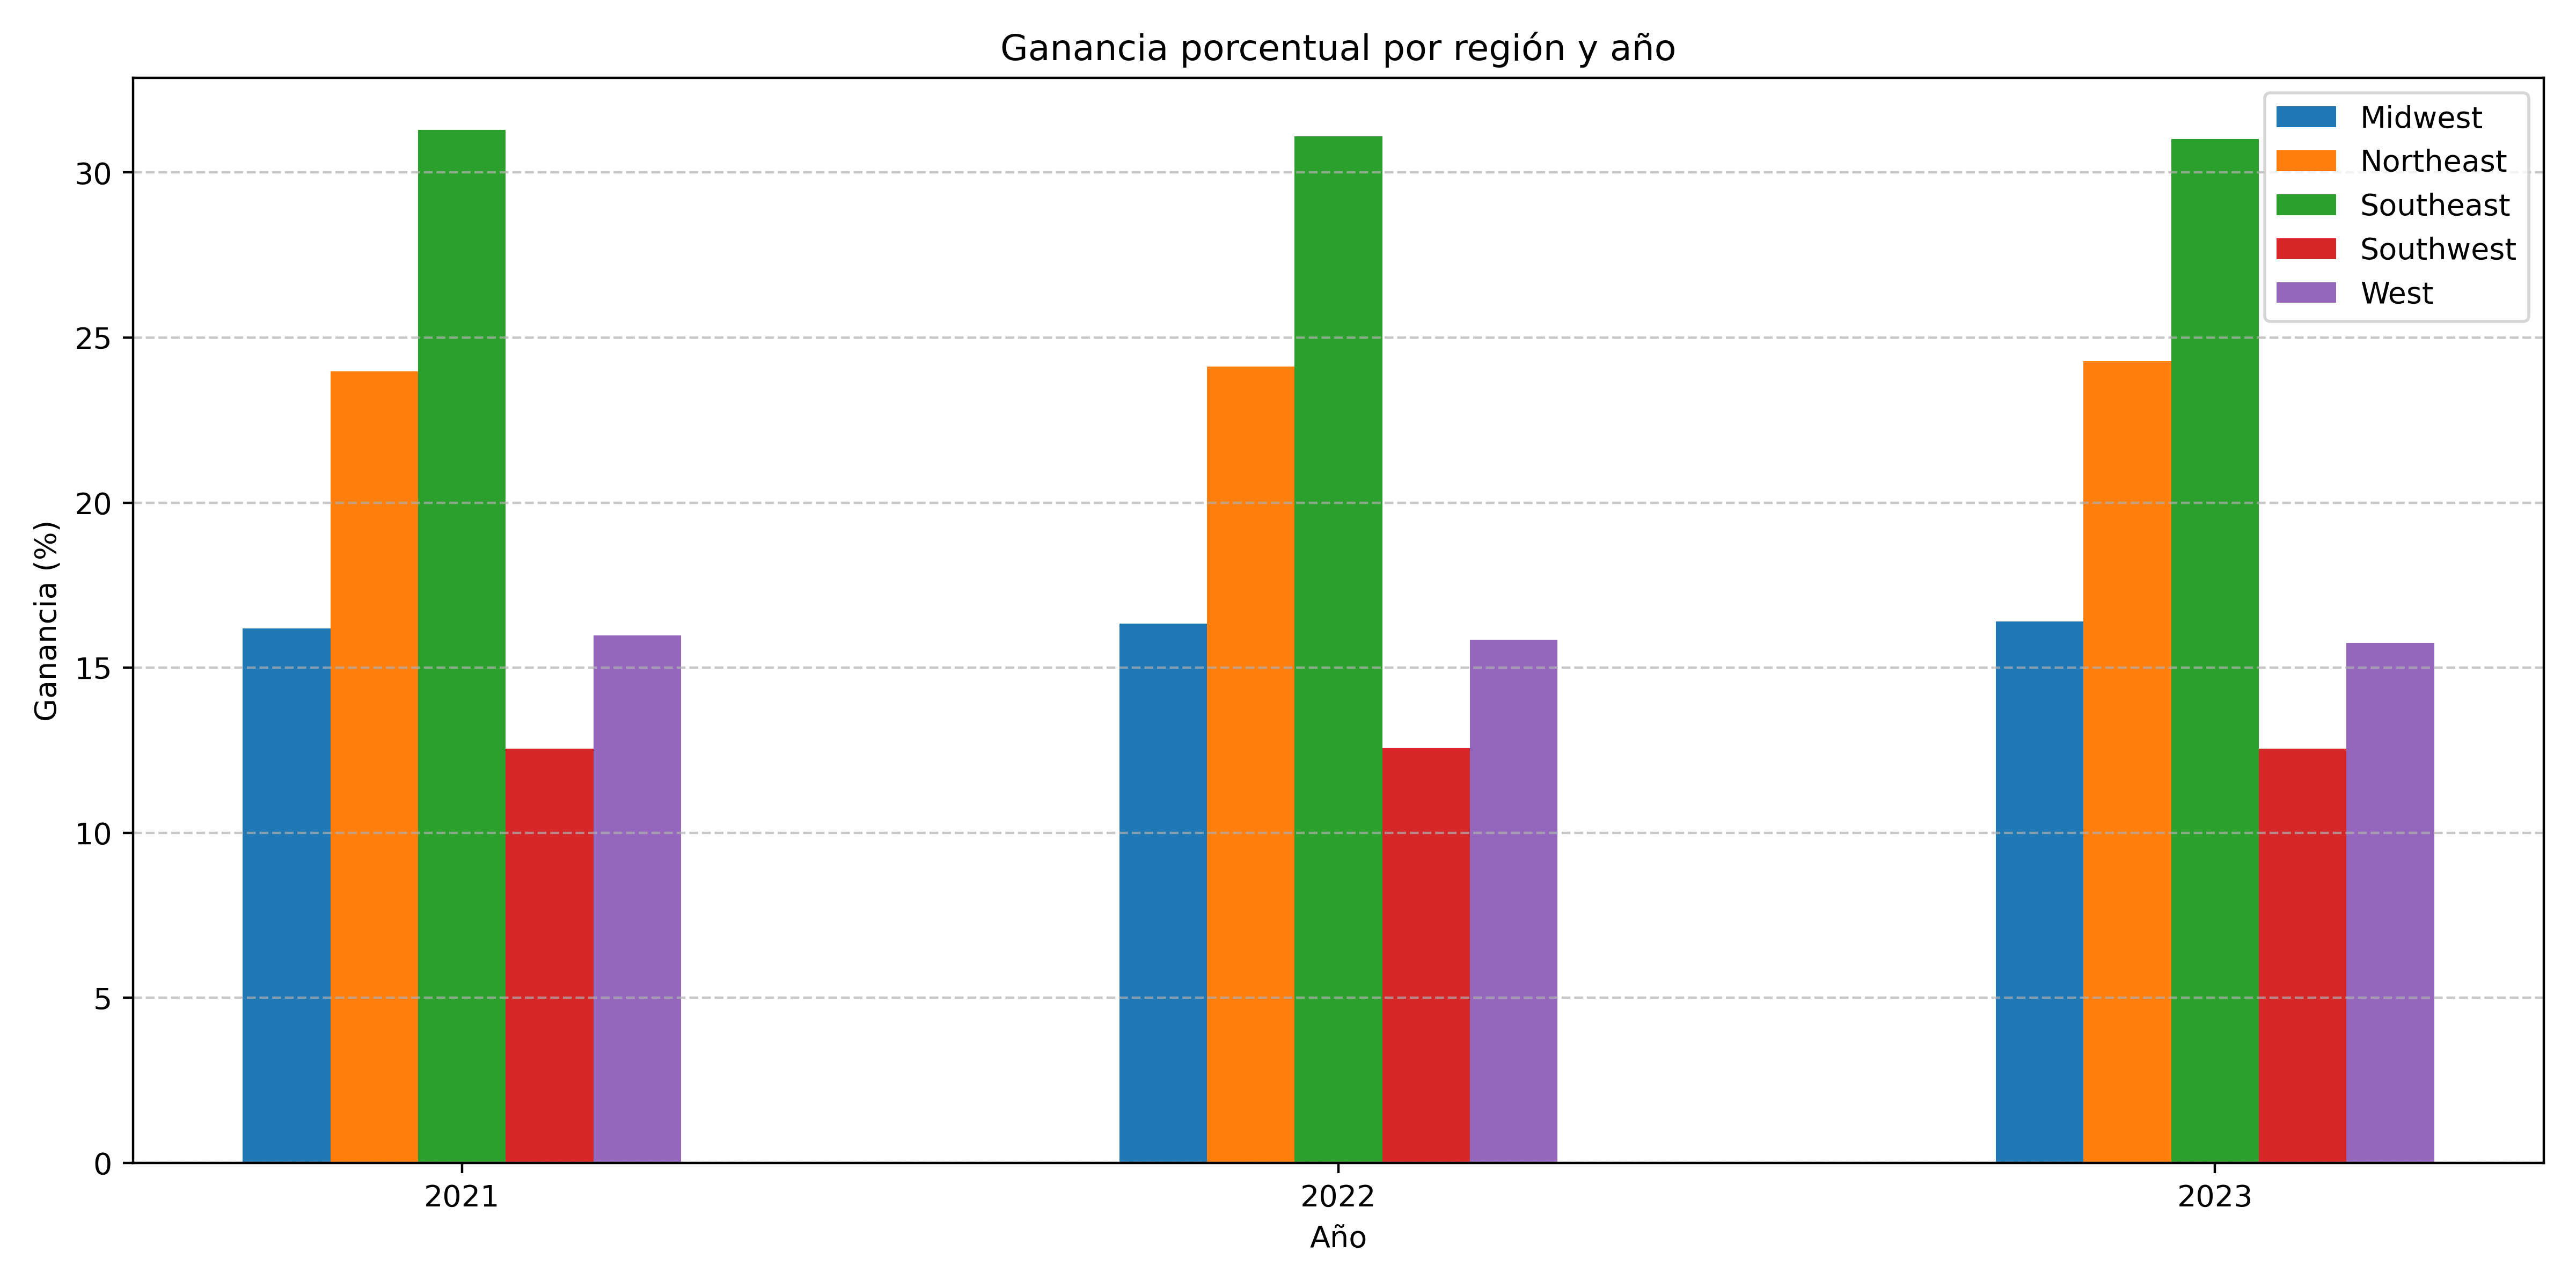
\includegraphics[width=0.8\textwidth]{graficos/ganancia_porcentual_por_region.png}%
    }
\end{center}

Antes de continuar, es importante aclarar que el subgrupo de productos de "Basketball" no registró ninguna venta en los últimos 3 años, lo que puede deberse 
a una falla en la carga de datos o a que el producto no se comercializa en las tiendas.

\vspace{0.2cm}

\newpage

La última observación que podemos hacer es que la demanda es muy sensible a los precios. Como se aprecia en el siguiente gráfico, 
la elasticidad en promedio es de aproximadamente 10, es decir, un aumento del 1\% en los precios implica una reducción del 
10\% en la demanda, y viceversa. Por lo tanto, cualquier estrategia de precios que se aplique debe tener en cuenta 
esta sensibilidad.

\begin{center}
    \makebox[\textwidth][c]{%
        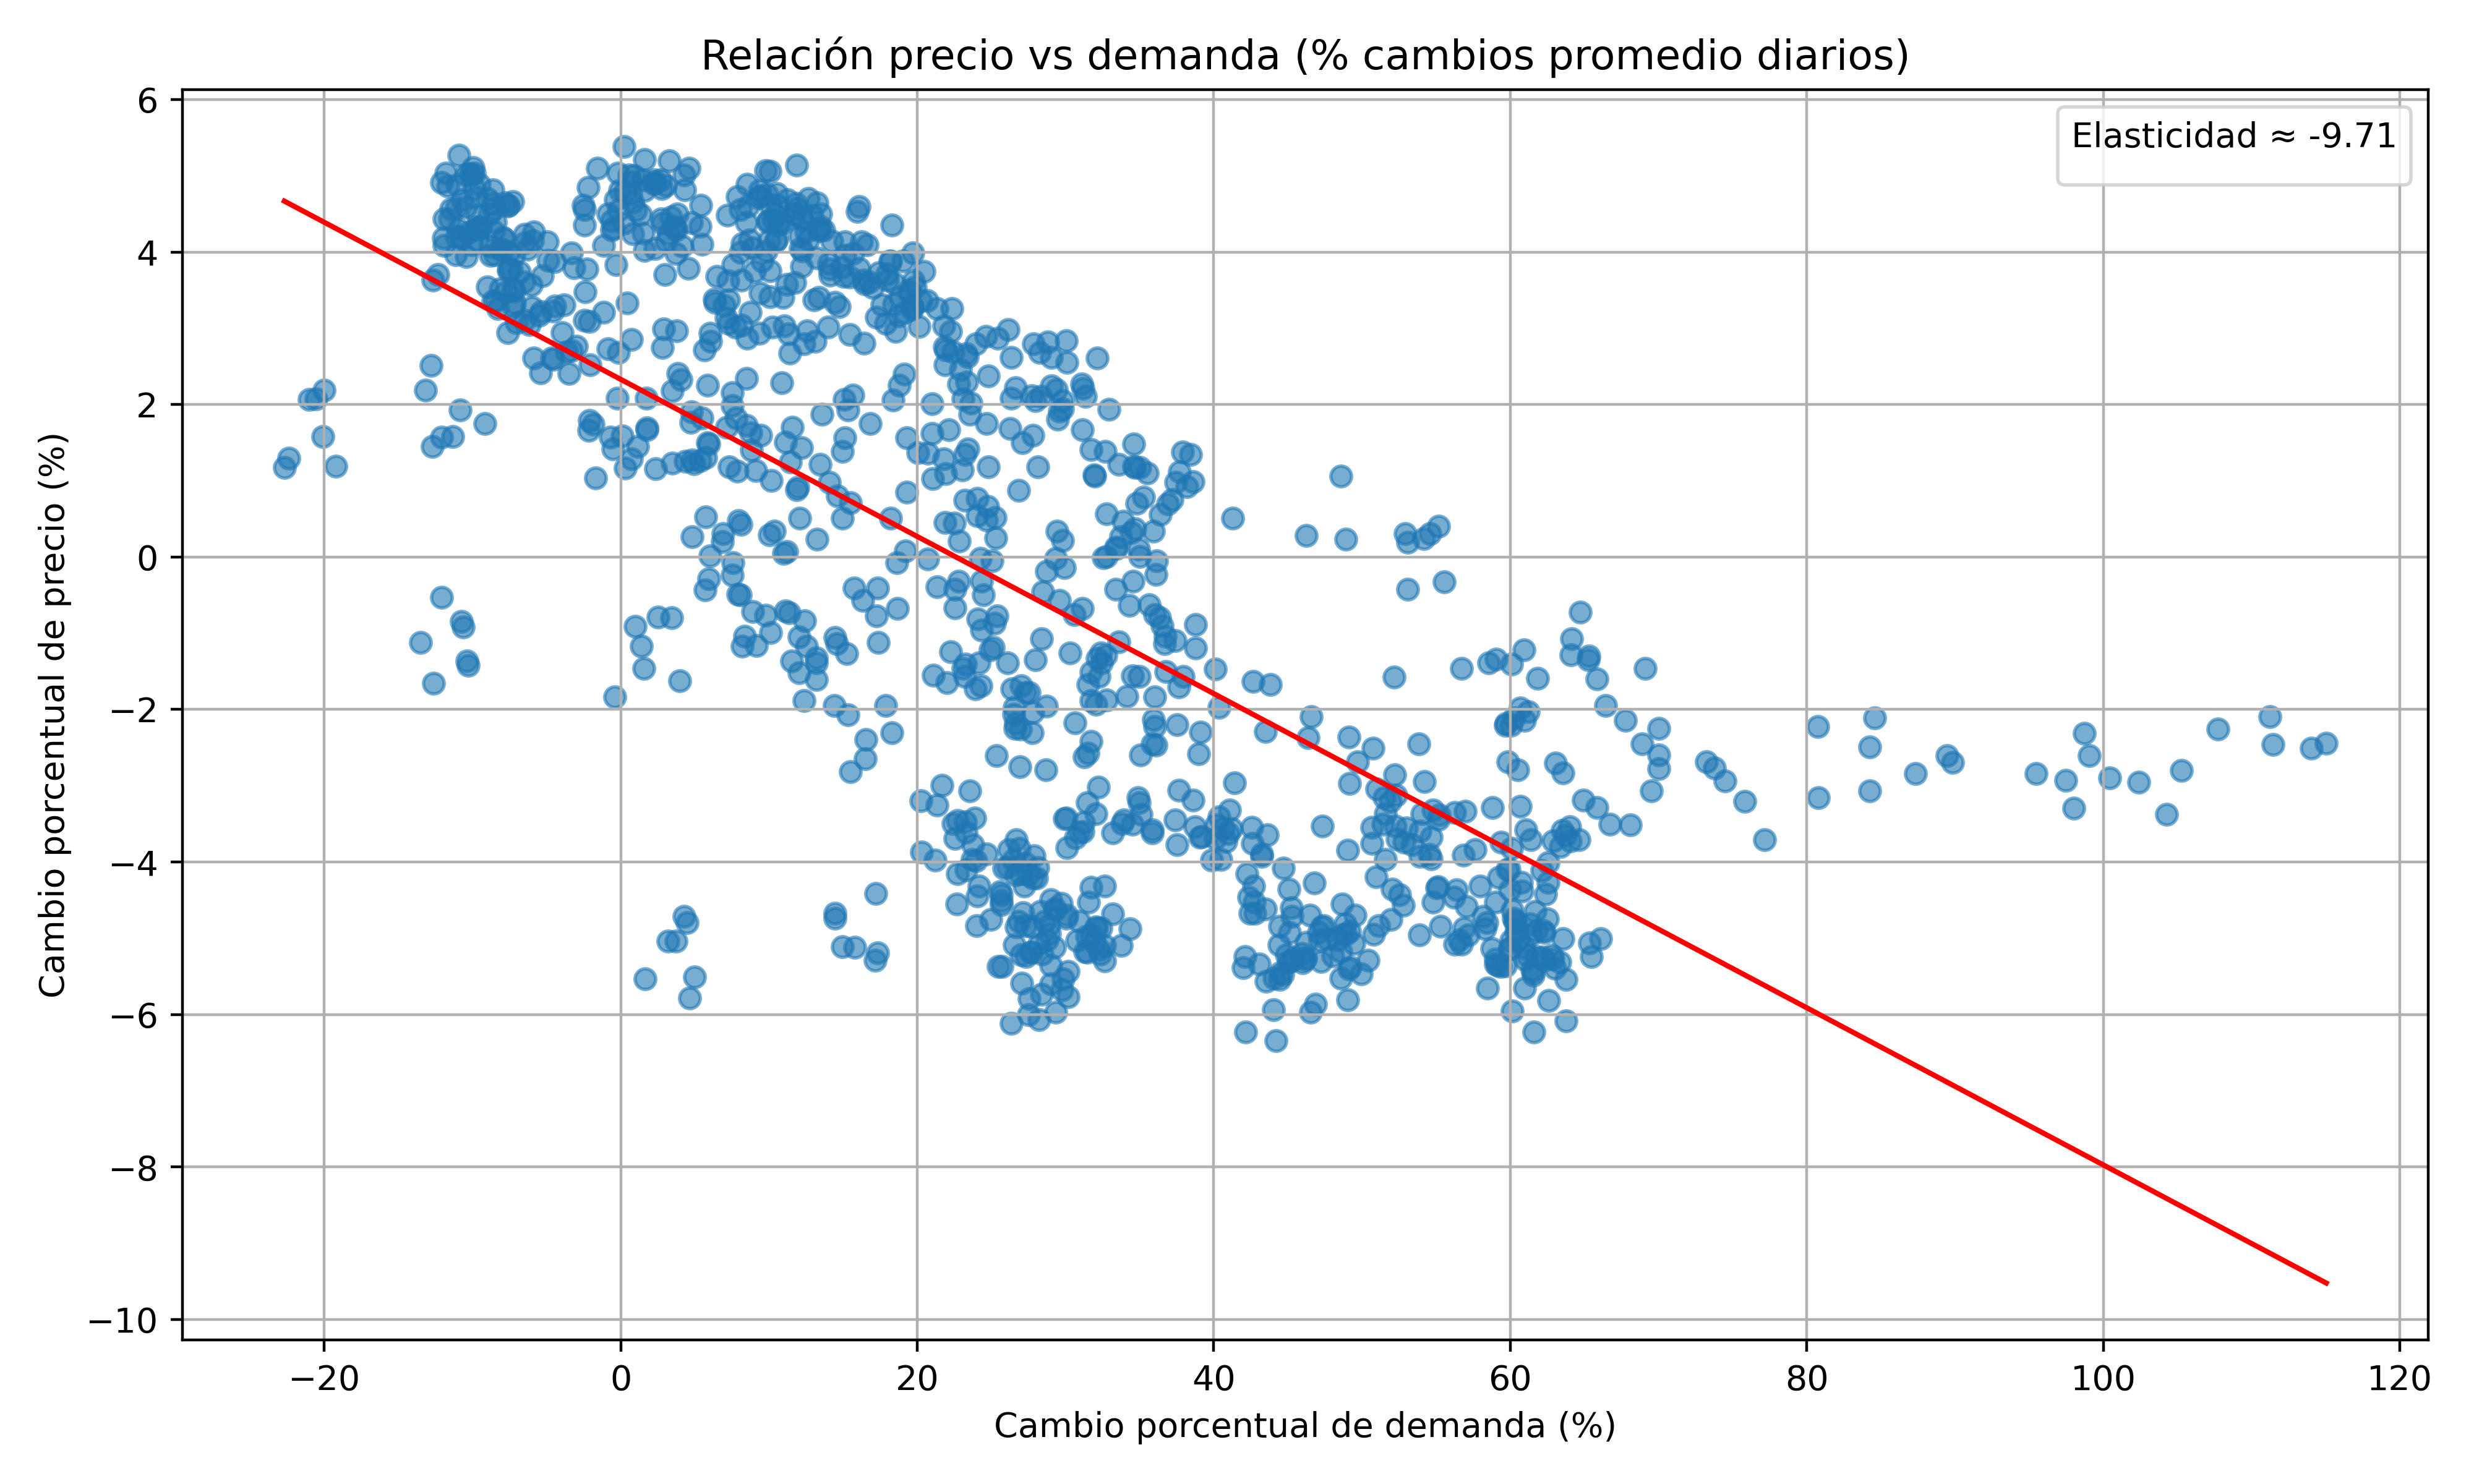
\includegraphics[width=0.8\textwidth]{graficos/relacion_precio_demanda.png}%
    }
\end{center}


Teniendo en cuenta todo lo anterior, construímos un modelo de inteligencia artificial capaz de predecir, con cierto margen 
de error, la demanda diaria de cada producto. De esta manera, pudimos simular qué precios serían los mejores para maximizar las ganancias de la próxima semana. 
Los mismos se encuentran en la carpeta "resultados" adjunto a este informe, en donde se indica para cada producto el precio óptimo. 

Además, para simplificar las modificaciones reales de los mismos, decidimos que todas las tiendas 
tengan el mismo precio para cada producto.

\vspace{0.2cm}

Veamos a grandes rasgos qué cambios se harían, viendo solamente en porcentaje promedio cuánto se debería 
aumentar o disminuir cada categoría:
\begin{center}
    \makebox[\textwidth][c]{%
        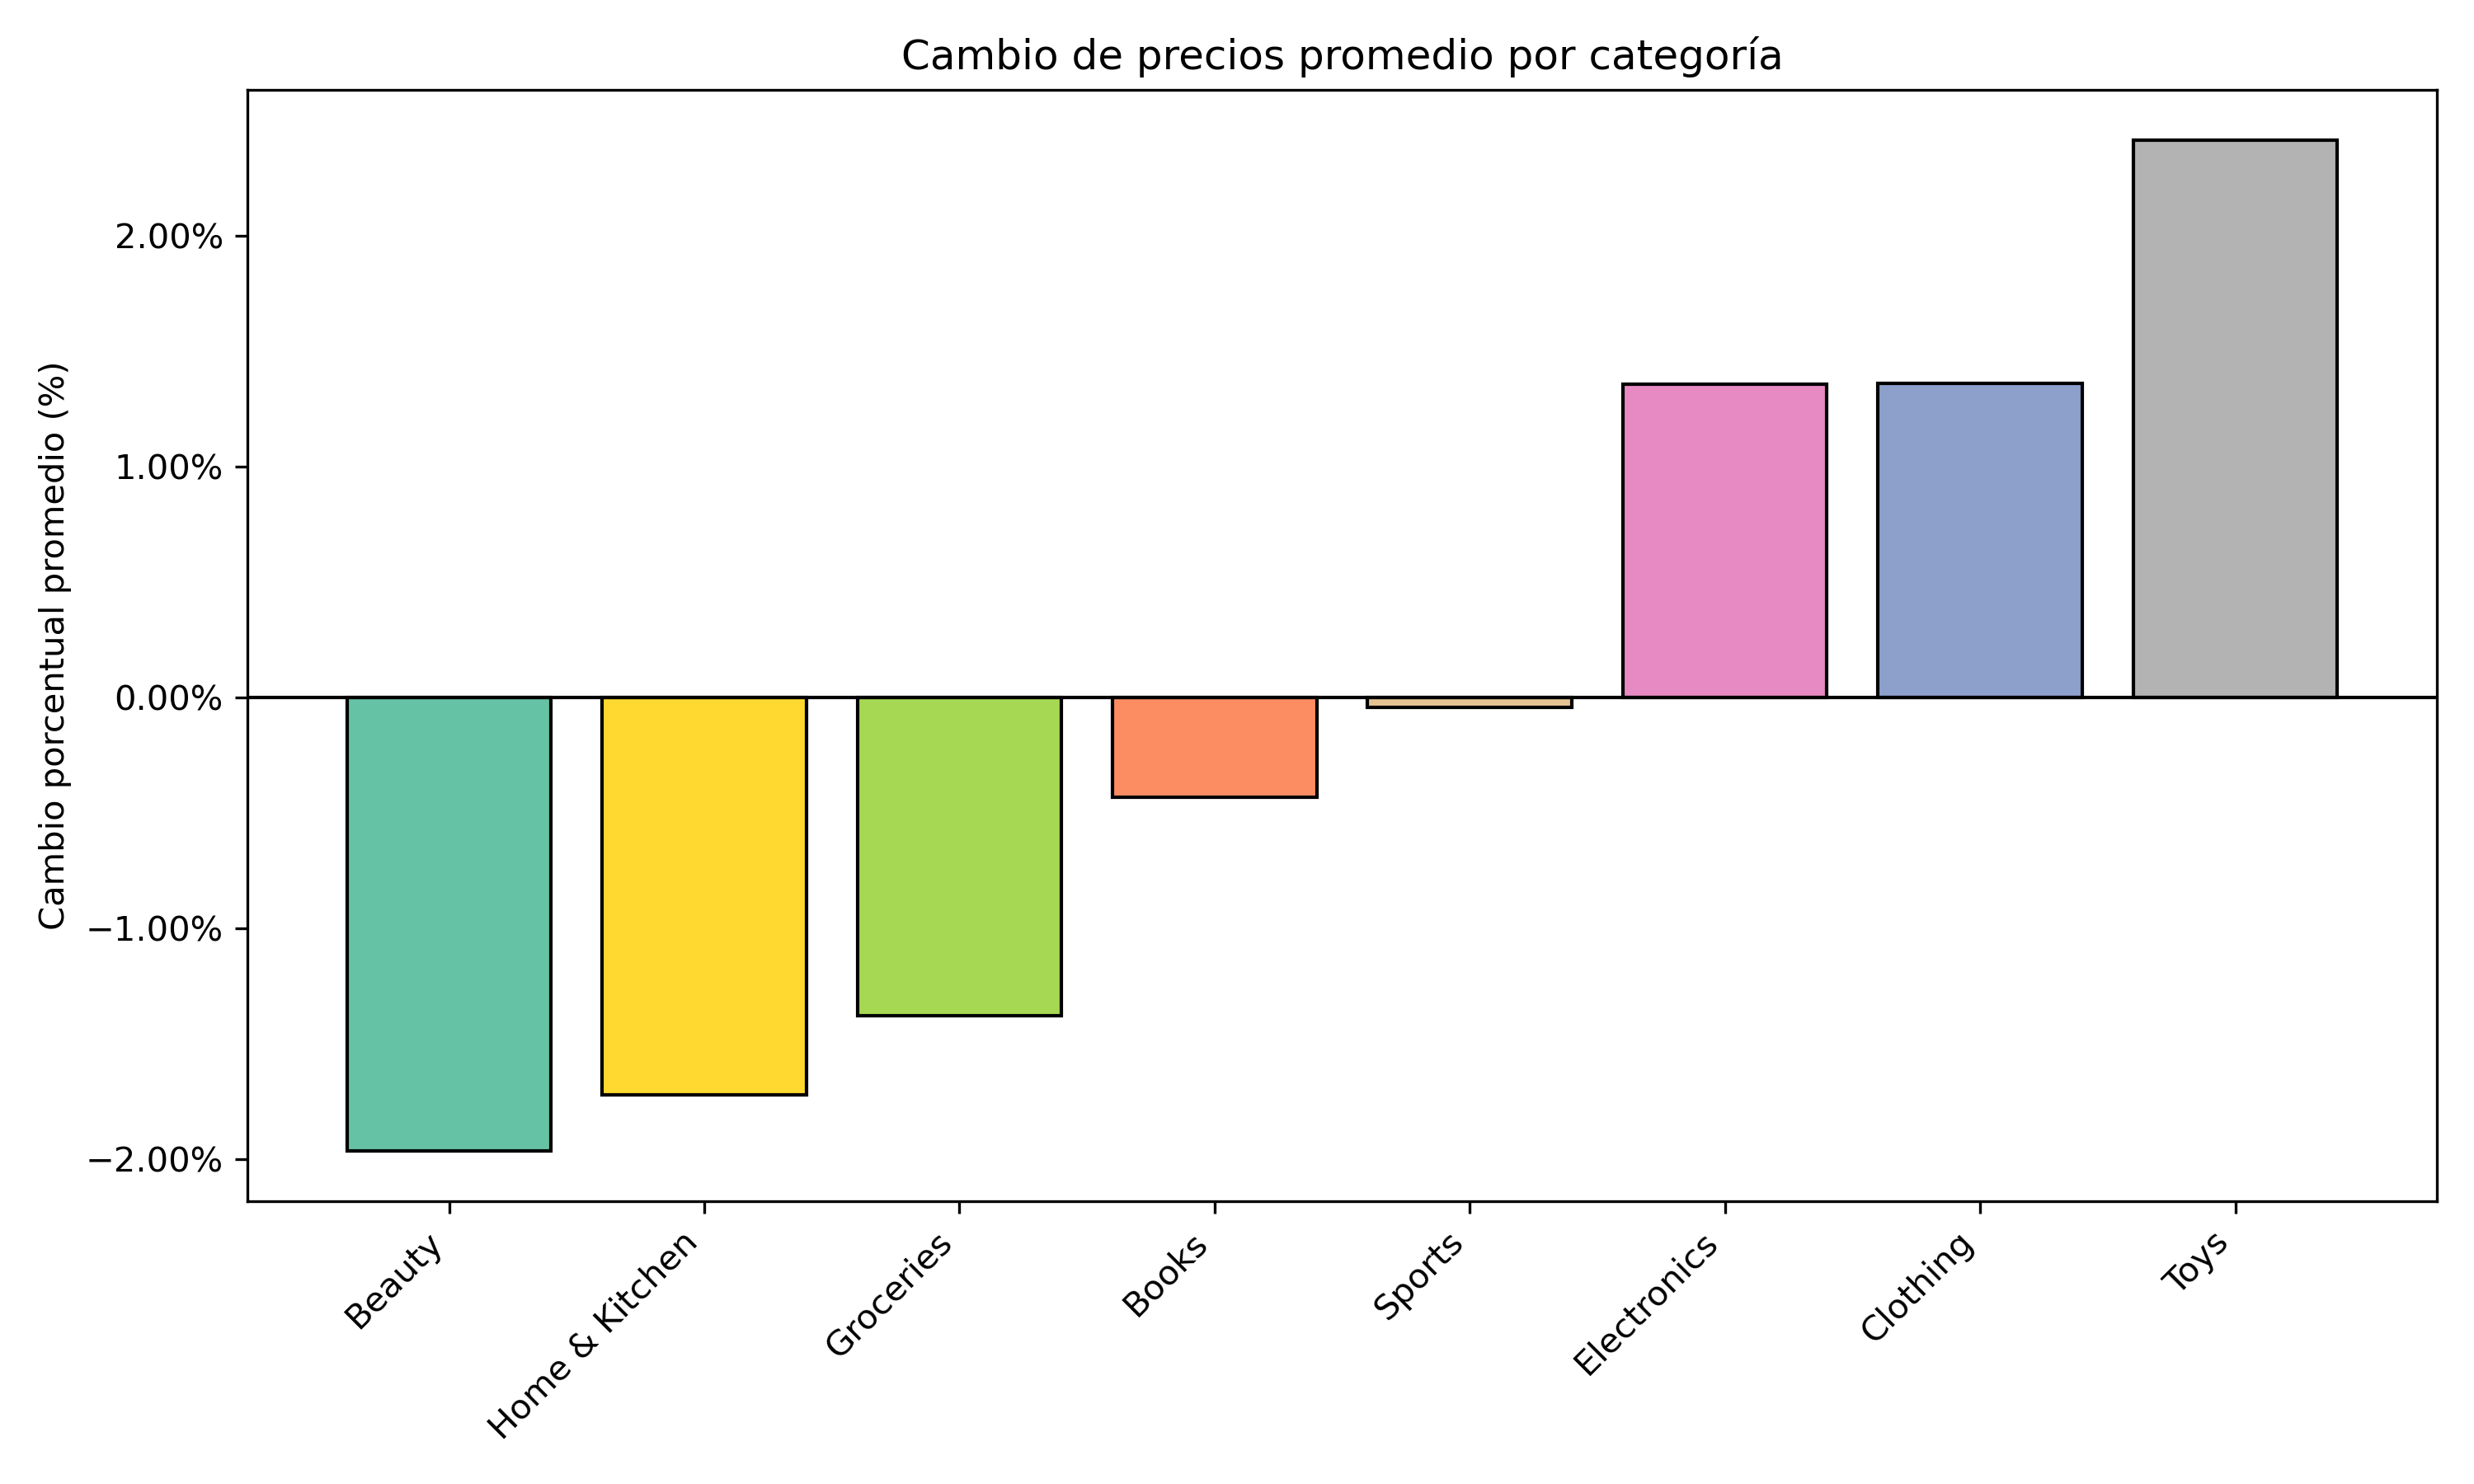
\includegraphics[width=0.8\textwidth]{graficos/cambios_nuevos_precios.png}%
    }
\end{center}

Podemos notar que los cambios no son tan significativos, dado que el máximo sólo supera por poco el 2\%. Sin embargo, 
las ventas esperadas sí se modifican sustancialmente: las ventas semanales promedio del último mes fueron de \$11.9 millones, 
mientras que las ventas esperadas por el modelo que empleamos con la configuración de precios propuesta es de \$16.7 millones, lo cual 
representa un aumento casi del 40\%. 

Por lo tanto, con esta metodología eventualmente se podría volver al nivel de ganancias del 2021, e incluso mejorarlo.










\newpage

\section{Análisis Técnico}

\subsection{Preprocesamiento de Datos}

Comenzamos el trabajo explorando los datos proporcionados y completando los datos faltantes. Después, nos quedamos con aquellas 
columnas que consideramos relevantes para el modelo e intentamos unir los 6 archivos csv en un mismo dataframe, sin embargo, 
los datos de los clientes no pudieron ser utilizados dado que las transacciones no contaban con el ID de cliente, por lo que no 
fue posible unirlos. 

\vspace{0.2cm}

Entonces, nos quedamos con los siguientes datos para cada transacción: fecha, producto (SKU), tienda, 
precio, costo, cantidad vendida (en unidades y en total), categorías del producto y ubicación de la tienda, entre otros.

\vspace{0.2cm}

Por otro lado, descartamos ciertos outliers que consideramos que podían llegar a cesgar al modelo: transacciones con precios, 
cantidad vendida unitaria o cantidad vendida total fuera del 99.9\% quantile.

\vspace{0.2cm}

\subsection{Análisis de Correlación entre Subgrupos}

En un principio, consideramos entrenar un modelo especializado para cada serie SKU-tienda o subgrupo-tienda. Esto tendría como ventaja modelos más simples, pero la desventaja era perder información cruzada entre grupos. Esto nos llevó a preguntarnos si existía correlación entre dichos grupos.  
Si los mismos fueran independientes, no habría relación cruzada y tendría sentido entrenar un modelo especializado por serie. 

Para evaluarlo, primero calculamos la correlación de Pearson, la cual mide relaciones lineales, y vimos que pocos subgrupos estaban fuertemente correlacionados.  
Sin embargo, como Pearson sólo captura correlaciones lineales, decidimos calcular también la correlación de Spearman y Kendall, métricas que permiten detectar relaciones monótonas entre variables, es decir, si tienden a moverse en la misma dirección aunque no sean lineales.  
Este análisis mostró que en gran cantidad de grupos sí existía correlación, ya sea directa o inversa. Por lo tanto, concluimos que ignorar estas interacciones no sería lo más adecuado, y optamos por entrenar un modelo global capaz de captarlas y generalizarlas.

\subsection{Modelo Predictivo}

    \subsubsection{Exploración de modelos}

    En una primera instancia, realizamos una etapa de investigación en la cual buscamos qué modelos se implementan en la industria para abordar la problemática de pronóstico de demanda y estrategia de precios. Decidimos probar al menos un 
    modelo de cada una de las siguientes familias: Regresiones, Boosting y Deep Learning.

    A continuación, se describen los distintos enfoques y pruebas realizadas durante esta etapa de exploración.

    \newpage

        \subsubsection{Regresiones}

        Como primera aproximación, entrenamos dos regresiones: una lineal y una polinomial. Estos modelos, al no ser estrictamente de series temporales, permitían que no fuera necesario completar el dataset con los días en que no hubo ventas 
        de un producto. Aun así, probamos agregar lagging features para que el modelo captara mejor la dinámica temporal: medias móviles y desviaciones estándar calculadas sobre datos anteriores, en diferentes ventanas de tiempo, agrupadas por subgrupo o por serie SKU-tienda, y considerando o no los datos faltantes.  
        También evaluamos distintas codificaciones para variables categóricas, incluyendo One-Hot Encoding y Target Encoding, siendo esta última preferida por reducir el tamaño del dataset codificado.

        Sin embargo, como era de esperar, la performance de estos modelos fue muy baja y decidimos descartarlos y probar modelos más complejos.

        \subsubsection{Deep Learning}

        Para la familia de Deep Learning, experimentamos con algunos modelos de la librería PyTorch Forecasting, que ofrece modelos muy potentes especializados en series temporales. 
        Además, permite el manejo de embeddings aprendidos para variables categóricas, lo cual resultaba ideal para nuestro problema, puesto que por la cantidad de categorías distintas un One-Hot Encoding aumenta demasiado la dimensionalidad del problema.
        
        \vspace{0.2cm}

        De esta librería probamos el modelo NHITS, que se basa en la descomposición de series para realizar predicciones. Sin embargo, esta no fue nuestra solución final debido a algunas problemáticas. Al tratarse de modelos para series temporales, el modelo 
        necesitaba ver todas las series completas (es decir, los días en que no hubo ventas para 
        cada producto y cada tienda). Así, terminábamos con un dataset muy grande con muchas series temporales, por que el entrenamiento del modelo era bastante costoso y difícil de efectuarle un fine-tuning adecuado. 
        Por lo tanto, decidimos probar modelos más simples y fáciles de entrenar, como los de la familia de Boosting.
        \vspace{0.2cm}

        \subsubsection{Boosting}

        El modelo que mejores resultados nos proporcionó fue el LightGBM, el cual es un modelo de boosting que utiliza árboles de decisión y 
        es capaz de manejar grandes volúmenes de datos de manera eficiente.

        \vspace{0.2cm}

    En primera instancia, utilizamos las transacciones dadas para entrenar el modelo, pero esto provocaba que después a la hora de 
    predecir la demanda por producto y tienda, el modelo no tuviera en cuenta los días en que no hubo ventas y sobreestimara por mucho 
    la demanda. Por lo tanto, decidimos crear un dataframe con todas las combinaciones posibles de fechas, productos y tiendas, y completar 
    los días en que no hubo ventas con un valor 0 en la cantidad vendida total.

    \vspace{0.2cm}

    Además, a partir del dataframe completo, para que el modelo pueda entender mejor la estacionalidad de la demanda, 
    creamos nuevos lagging features: agrupamos las transacciones por producto y calculamos 
    una media móvil de la cantidad vendida total y su desviación estándar de los últimos días, para distintas ventanas temporales. 
    Hicimos lo mismo pero agrupando por tienda, como también por subgrupo de productos.

    \vspace{0.2cm}

    Por otro lado, para que el modelo pueda relacionar mejor el precio y la demanda, creamos otros lagging features sobre los precios: 
    agrupando las transacciones por producto, calculamos la media móvil y desviación estándar del cambio porcentual del precio de los 
    últimos días, para distintas ventanas temporales. También hicimos lo mismo, pero agrupando por subgrupo de productos.

    \vspace{0.2cm}

    Entonces, con el dataframe completo y los features agregados, comenzamos a probar el modelo. Para esto, no podíamos emplear un cross-validation 
    convencional, dado que los lagging features hubieran generado data leakage, por lo que decidimos hacer un walk-forward validation: 
    entrenar el modelo con los datos del primer año, predecir la demanda de la próxima semana, guardar las predicciones y compararlas con 
    las ventas reales, y luego sumar 30 días a los datos de entrenamiento y repetir el proceso. De esta manera, podemos evaluar la performance del 
    modelo prediciendo la demanda de la próxima semana, tal como se haría si tuviéramos que hacerlo en tiempo real.

    \vspace{0.2cm}

    El fine-tuning del modelo se debió hacer de manera manual, puesto que el entrenamiento de cada modelo tenía un gran costo computacional 
    y, por lo tanto, un Grid Search no era viable con los recursos disponibles.



\subsection{Optimización de Precios}

Después de validar el modelo, elegimos los hiperparámetros que mejor performance nos dieron y entrenamos el modelo con todos los datos 
disponibles. Luego, creamos un dataframe template con todas las combinaciones posibles de fechas, productos y tiendas de la próxima semana, 
exluyendo las tiendas que cerraron. 

\vspace{0.2cm}

Debido a que probar todas las configuraciones de precios posibles para predecir cuál maximiza las ventas totales era computacionalmente inviable, primero 
redujimos el espacio de búsqueda: para cada producto, quitamos los precios que se apartaban demasiado del rango de los últimos días. Tomando como ejemplo 
los precios de BEAHASH009, ya vistos anteriormente, podemos ver a continuación los precios filtrados:

\begin{center}
    \makebox[\textwidth][c]{%
        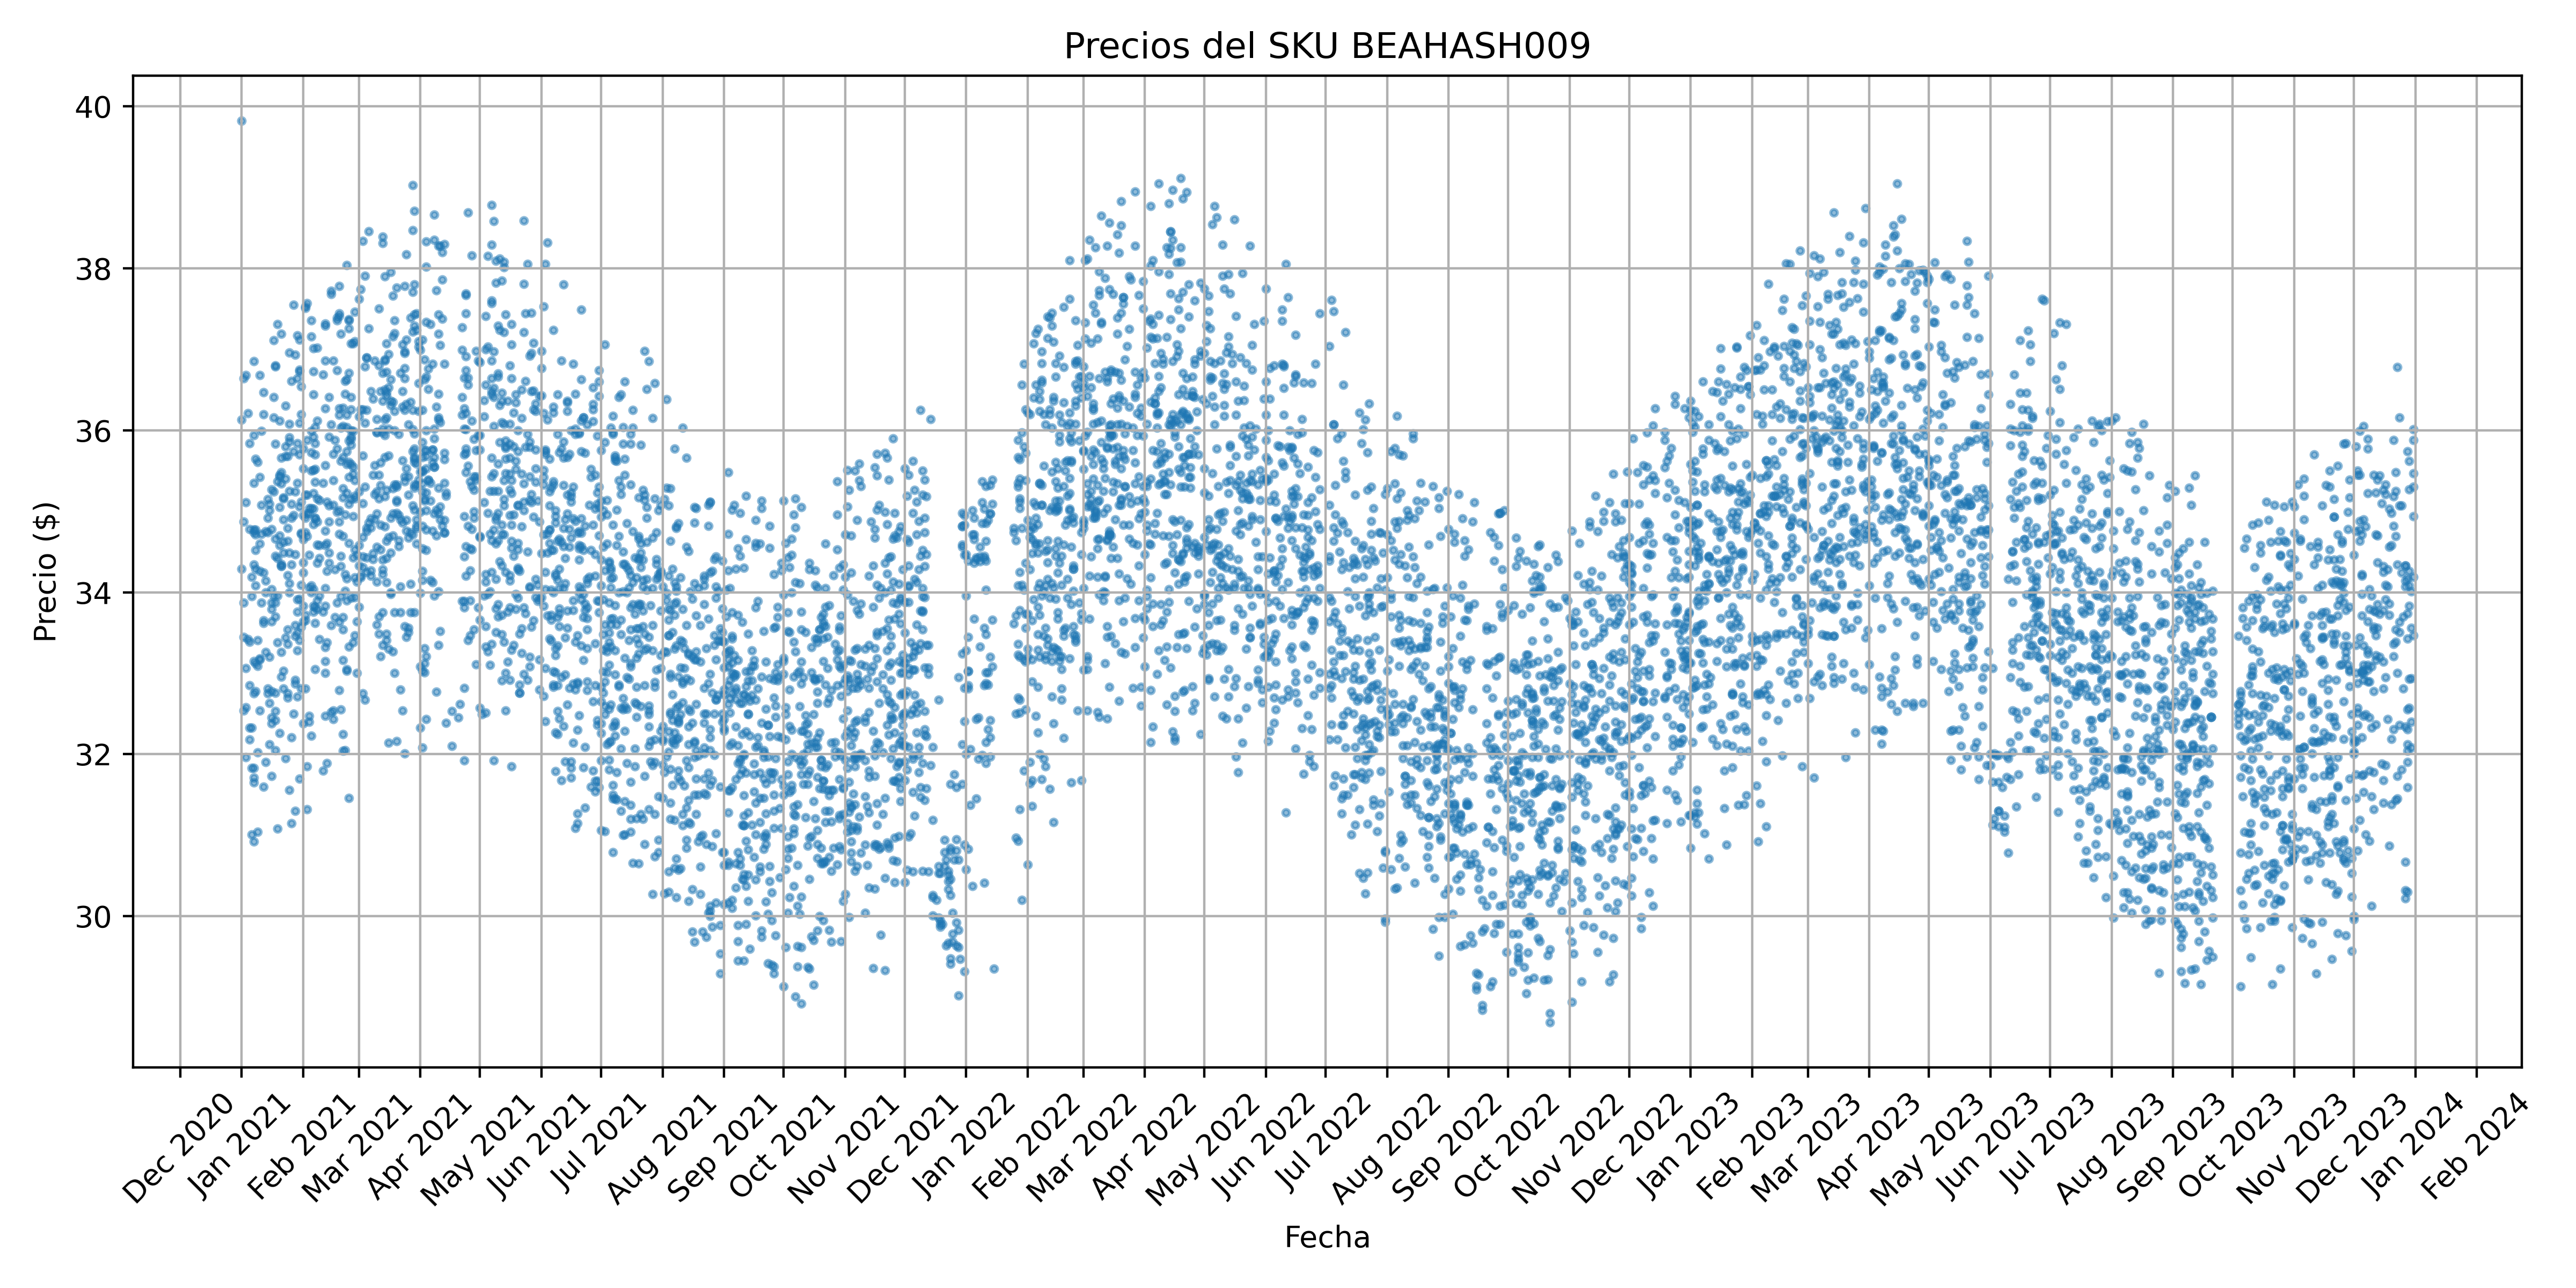
\includegraphics[width=1\textwidth]{graficos/precios_sku_BEAHASH009_filtrado.png}%
    }
\end{center}

\newpage

Entonces, tomamos como rango de precios posibles para cada producto el máximo y el mínimo de los precios filtrados en los últimos 30 días. Cabe aclarar que 
aún así los datos con los precios no filtrados sí fueron utilizados para entrenar el modelo.

\vspace{0.2cm}

Además, para simplificar la implementación de la estrategia de precios, decidimos que los precios de los productos serán los mismos en todas las tiendas y 
para toda la semana (aunque también probamos cambiar los precios por región, pero no mejoró los resultados).

\vspace{0.2cm}

Así, con un espacio de búsqueda más manejable, aplicamos una optimización bayesiana (con la librería Optuna) para encontrar la configuración de precios 
que maximiza las ventas totales según las predicicones del modelo. También probamos maximizar las ganancias totales (es decir, las ventas menos los costos), aunque 
el resultado muy similar.

\vspace{0.2cm}

Como ya expusimos anteriormente, los resultados fueron muy positivos, y se esperaría aumentar casi un 40\% las 
ventas semanales.


\subsection{Interpretación del modelo}

Gracias a que empleamos un modelo basado en árboles de decisión y no en redes neuronales complejas, nuestro modelo es altamente interpretable. 
Veamos a continuación qué features fueron los más relevantes para la mejora de la performance del LightGBM: 

\begin{center}
    \makebox[\textwidth][c]{%
        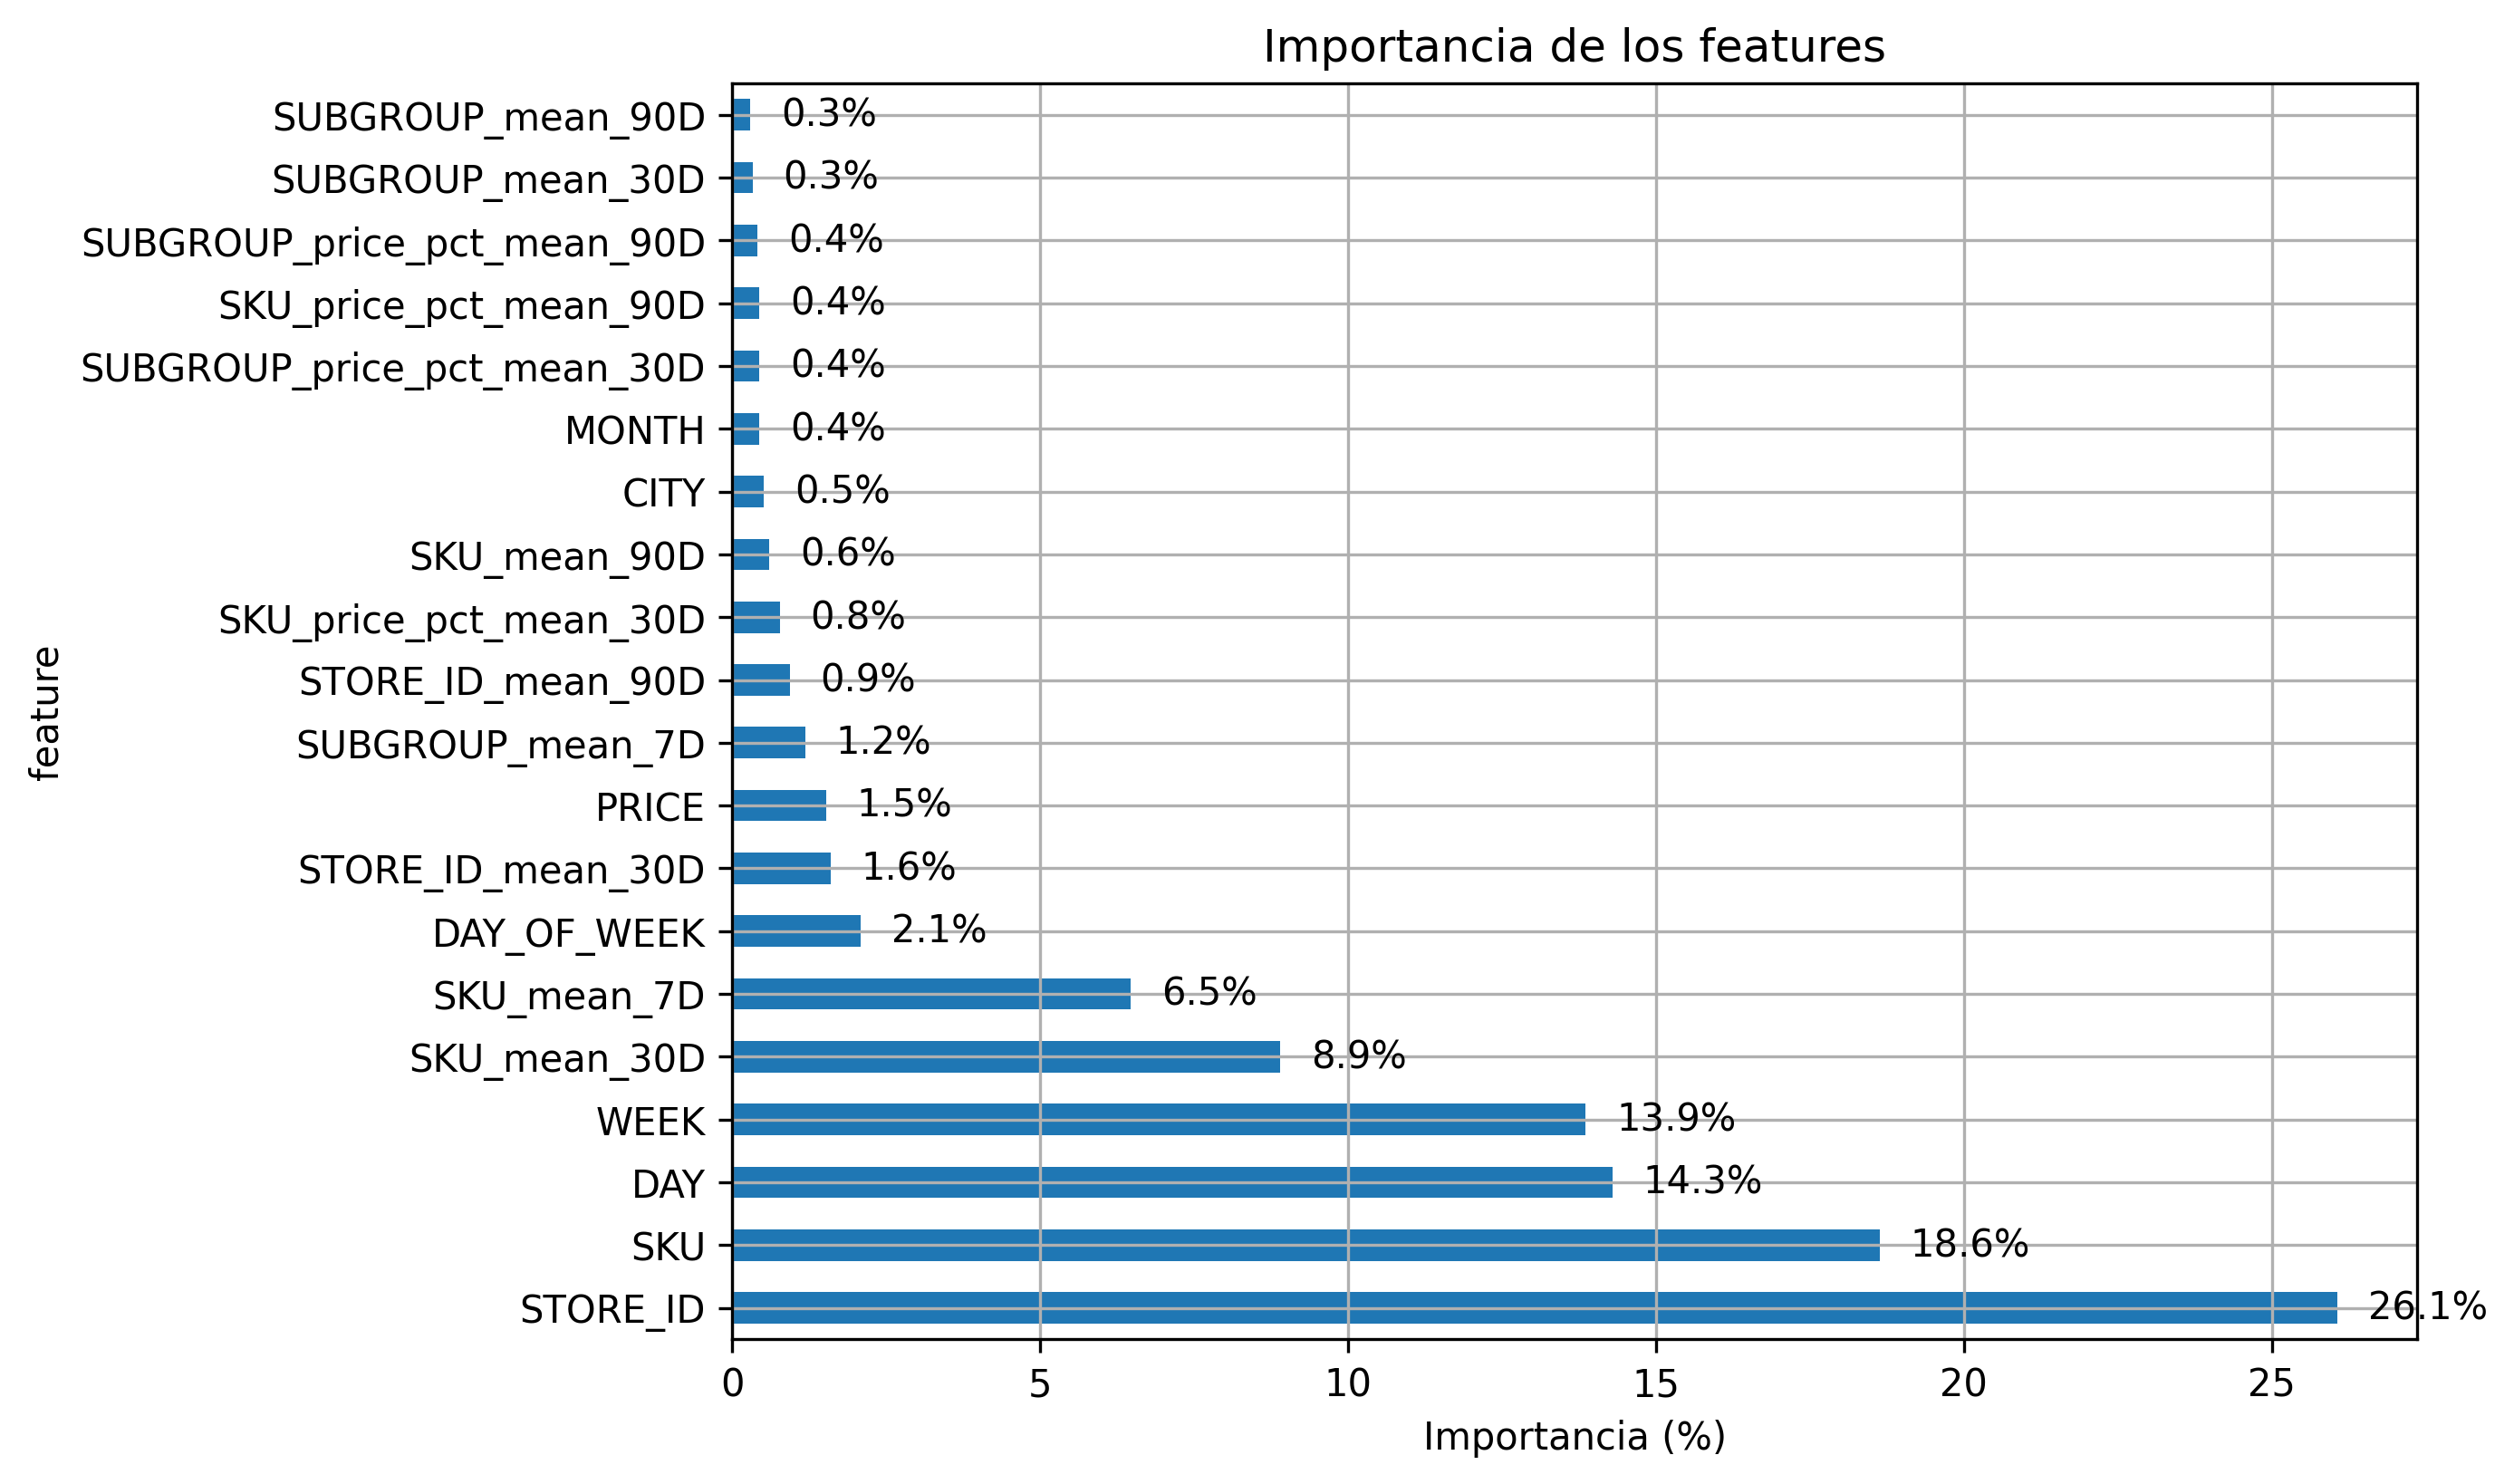
\includegraphics[width=1\textwidth]{graficos/importancia_features.png}%
    }
\end{center}

Aclaración sobre el formato de los features: SUBGROUP\_price\_pct\_mean\_30D se refiere a la media móvil de los últimos 30 días 
del cambio porcentual de los productos agrupados por la columna SUBGROUP, mientras que SUBGROUP\_mean\_30D se refiere a la misma media móvil 
pero de las ventas totales.

\vspace{0.2cm}

De esta manera, podemos concluir que el modelo pudo captar lo importante que es el momento del año para predecir las ventas, como también lo fue 
conocer el producto, sin importar tanto a qué categoría pertenecía. 

\vspace{0.2cm}

Además, un detalle interesante es que al ser STORE\_ID el feature más relevante, 
esto quiere decir que las ventas cambian drásticamente según la tienda, como ya habíamos anticipado cuando analizamos el porcentaje de ganancias por región. 
Sabiendo esto, lo más adecuado sería intentar optimizar los precios no sólo por región, sino por tienda. Sin embargo, esto sería muy costoso computacionalmente.

\vspace{0.2cm}

También fue de gran utilidad los lagging features para reconocer los patrones de ventas estacionales, tanto de los productos, subgrupos y tiendas. Cabe destacar 
que fueron incluso más importantes que las mismas categorías del producto.

\vspace{0.2cm}

Otro punto para resaltar es que el precio tenga tanta poca importancia. Debido a esto, uno podría dudar de si realmente el modelo 
está captando adecuadamente la relación precio-demanda. Aún así, durante la optimización fue claro que el modelo cambiaba significativamente sus 
predicciones según los precios, manteniendo el resto de variables fijas.






\newpage

\section{Consideraciones Finales}

En resumen, se pudo dar un análisis que dio un panorama de la situación actual de la empresa: cómo 
fueron reduciendo sus ganancias y cuáles fueron los motivos más probables. A partir de esto, utilizamos un 
modelo de AI que fue capaz de captar los patrones de la demanda y así construir una nueva estrategia de precios 
maximizando las ganancias. 

\vspace{0.2cm}

Aunque los resultados sean buenos, dado que un aumento esperado del 40\% de las ganancias es muy significativo, es 
importante aclarar que los modelos predictivos siempre tienen un margen de error y estos aumentos de ventas 
nunca pueden estar garantizados. Aún así, creemos que es una buena aproximación, basada en un arduo análisis 
y experimentación, que puede beneficiar en gran medida a la empresa.

\vspace{0.2cm}

Para un trabajo futuro, se debe considerar si los productos del subgrupo Basketball realmente no fueron 
vendidos, y si fue así y no se debe a una falla en la carga de datos, sugerimos evaluar la posibilidad de retirar estos 
productos del catálogo. 

\vspace{0.2cm}

Finalmente, si la empresa está satisfecha con esta primera aproximación de una estrategia de precios óptima, 
podríamos mejorarla si se nos permite modificar los precios de un mismo producto en distintas tiendas, 
en el caso de que sea factible en términos administrativos.

\end{document}
